\documentclass[11pt]{article}

\usepackage[a4paper,margin=2cm]{geometry}
\usepackage{upquote,amsmath,natbib,sidecap,caption}
\usepackage[svgnames]{xcolor}
\usepackage[most]{tcolorbox}

\makeatletter
\def\bbordermatrix#1{\begingroup \m@th
  \@tempdima 4.75\p@
  \setbox\z@\vbox{%
    \def\cr{\crcr\noalign{\kern2\p@\global\let\cr\endline}}%
    \ialign{$##$\hfil\kern2\p@\kern\@tempdima&\thinspace\hfil$##$\hfil
      &&\quad\hfil$##$\hfil\crcr
      \omit\strut\hfil\crcr\noalign{\kern-\baselineskip}%
      #1\crcr\omit\strut\cr}}%
  \setbox\tw@\vbox{\unvcopy\z@\global\setbox\@ne\lastbox}%
  \setbox\tw@\hbox{\unhbox\@ne\unskip\global\setbox\@ne\lastbox}%
  \setbox\tw@\hbox{$\kern\wd\@ne\kern-\@tempdima\left[\kern-\wd\@ne
    \global\setbox\@ne\vbox{\box\@ne\kern2\p@}%
    \vcenter{\kern-\ht\@ne\unvbox\z@\kern-\baselineskip}\,\right]$}%
  \null\;\vbox{\kern\ht\@ne\box\tw@}\endgroup}
\makeatother

\title{Exploratory analysis of provenance data\\ using \texttt{R} and
  the \texttt{provenance} package}

\author{Pieter Vermeesch\\
  University College London\\
  Gower Street, London WC1E 6BT\\
  United Kingdom\\
  \texttt{p.vermeesch@ucl.ac.uk}
}

\date{}

\setlength{\parindent}{0pt}

\begin{document}

\maketitle

\begin{abstract}
  The provenance of siliclastic sediment may be traced using a wide
  variety of chemical, mineralogical and isotopic proxies. These
  define three distinct data types: (1) compositional data such as
  chemical concentrations; (2) point-counting data such as heavy
  mineral compositions; and (3) distributional data such as zircon
  U-Pb age spectra. Each of these three data types requires separate
  statistical treatment. Central to any such treatment is the ability
  to quantify the `dissimilarity' between two samples. For
  compositional data, this is best done using a logratio
  distance. Point-counting data may be compared using the chi-square
  distance, which deals better with missing components (zero values)
  than the logratio distance does. Finally, distributional data can be
  compared using the Kolmogorov-Smirnov and related statistics.\\

  For small datasets using a single provenance proxy, data
  interpretation can sometimes be done by visual inspection of ternary
  diagrams or age spectra. But this no longer works for larger and
  more complex datasets. This paper reviews a number of multivariate
  ordination techniques to aid the interpretation of such
  studies. Multidimensional Scaling (MDS) is a generally applicable
  method that displays the salient dissimilarities and differences
  between multiple samples as a configuration of points in which
  similar samples plot close together and dissimilar samples plot far
  apart.  For compositional data, classical MDS analysis of logratio
  data is shown to be equivalent to Principal Component Analysis
  (PCA). The resulting MDS configurations can be augmented with
  compositional information as biplots. For point-counting data,
  classical MDS analysis of chi-square distances is shown to be
  equivalent to Correspondence Analysis (CA). This technique also
  produces biplots.\\

  Thus, MDS provides a common platform to visualise and interpret all
  types of provenance data. Generalising the method to three-way
  dissimilarity tables provides an opportunity to combine several
  multi-method datasets together and thereby facilitate the
  interpretation of `Big Data'.  This paper presents a set of
  tutorials using the statistical programming language \texttt{R}. It
  illustrates the theoretical underpinnings of compositional data
  analysis, PCA, MDS and other concepts using toy examples, before
  applying these methods to real datasets with the \texttt{provenance}
  package.
\end{abstract}

\section{Introduction}

At its most basic level, sedimentary provenance analysis identifies
the mineralogical, chemical or isotopic composition of individual
grains, or assemblages of multiple grains in siliclastic
sediment. These properties can then be used to group samples of
similar affinity, and thereby trace the flow of sediment through a
sediment routing system \citep[e.g.,][]{morton1991, weltje2004,
  gerdes2006, rittner2016, mazumder2017}. Different levels of
statistical complexity arise when multiple samples are compared to
each other, or when multiple provenance proxies are applied to
multiple samples.\\

Using a number of short tutorials, this paper will introduce several
simple but effective exploratory data analysis techniques that can
help to make geological sense of `Big Data' in a sedimentary
provenance context. The term `exploratory' means that these techniques
allow the user to explore the data independent of any prior knowledge
about the geological setting \citep{tukey1977, dutoit1986, kenkel2006,
  martinez2017}.  It groups a number of graphical methods to visualise
the data and reveal patterns of similarity and differences between
samples and variables.  This paper will not introduce methods such as
discriminant analysis that formally assign samples to pre-defined
provenance areas or petrotectonic settings \citep{bhatia1983,
  bhatia1986}.\\

These notes do by no means pretend to give a comprehensive overview of
exploratory data analysis. The selection of methods presented herein
is heavily biased towards techniques that are implemented in a
software package for (sedimentary) geology that was created by
\citet{vermeesch2016a}.\\

\texttt{provenance} is available free of charge at the Comprehensive R
Archive Network (CRAN,
\texttt{http://cran.}\allowbreak\texttt{r-project.org/}\allowbreak\texttt{web/}\allowbreak\texttt{packages}),
on GitHub
(\texttt{http://github.}\allowbreak\texttt{com/pvermees/provenance}),
or via
\texttt{http://provenance.}\allowbreak\texttt{london-geochron.}\texttt{com}. The
package is written in the statistical programming language \texttt{R},
which is available for Windows, Mac OS-X and Linux/Unix. The easiest
way to install the latest stable version of the package is to first
install \texttt{R} from
\texttt{http://r-project.}\allowbreak\texttt{org} and then type the
following code at the command prompt (i.e. the `\verb|>|'):

%\begin{tcolorbox}
\begin{verbatim}
> install.packages('provenance')
\end{verbatim}
%%\end{tcolorbox}

Once installed, the package can be loaded by typing:

%\begin{tcolorbox}
\begin{verbatim}
> library(provenance)
\end{verbatim}
%\end{tcolorbox}

There are two ways to use \texttt{provenance}.  The first of these is
 through a query-based user interface. To access this interface, type:

 %\begin{tcolorbox}
\begin{verbatim}
> provenance()
\end{verbatim}
%\end{tcolorbox}

The main advantage of the query-based user interface is that it does
not require any knowledge of \texttt{R}. Its main disadvantage is the
relative lack of flexibility and the difficulty to automate complex
and/or repetitive tasks. The second way to use \texttt{provenance} is
via the \texttt{R} language itself. This is the quicker and more
flexible option, whose only downside is a steeper learning curve
compared to the query-based interface. This tutorial will help the
reader to climb this learning curve whilst explaining the theoretical
underpinnings of the methods that are implemented in the package.\\

This text assumes that the reader has a basic understanding of the
\texttt{R} programming language, although a short tutorial is provided
in the Appendix for readers who lack such prior knowledge. The paper
also assumes that the reader has some basic statistical
knowledge. More specifically (s)he is expected to be familiar with the
normal distribution, and understand the meaning of the arithmetic
mean, standard deviation and confidence intervals. The normal
distribution underpins much of `conventional' statistics, but we will
see that it rarely applies to provenance data.  This, in fact, is the
main take-home message of this paper.\\

There exist three fundamental types of provenance data:

\begin{enumerate}
  
\item Chemical data such as major and trace element concentrations are
  known as \emph{compositional} data. Sections~\ref{sec:ratios} and
  \ref{sec:compositional} show that the statistical analysis of this
  class of data is fraught with difficulties. Fortunately these are
  easily overcome by means of `Aitchison's logratio
  transformation'. This transformation is a prerequisite to further
  statistical treatment, including Principal Component Analysis and
  compositional biplots of multi-sample datasets
  (Sections~\ref{sec:ratios} and \ref{sec:compositional}).

\item Categorical data such as bulk petrography and heavy mineral
  compositions are known as \emph{point-counting} data. These are
  closely related to, but are fundamentally different from,
  compositional data. Compositional data consist of strictly positive
  real numbers that are subject to a constant-sum constraint and whose
  analytical precision can generally be ignored. In contrast,
  point-counting data contain integer values that may be greater than
  or equal to zero, and whose multinomial uncertainty is significant
  compared to the underlying compositional
  dispersion. Section~\ref{sec:counts} shows that both of these
  differences can be captured by a combination of logistic normal and
  multinomial statistics.

\item Detrital age spectra form a third class of data that will be
  referred to as \emph{distributional} data.
  Sections~\ref{sec:distributional} and \ref{sec:MDS} introduce kernel
  density estimation, the Kolmogorov-Smirnov statistic, and
  multidimensional scaling as ways to visualise, compare, and
  interpret distributional data.

\end{enumerate}

Finally, Section~\ref{sec:bigdata} will consider the case where
multiple compositional, point-counting and/or distributional datasets
are combined. Procrustes analysis and 3-way multidimensional scaling
are statistical techniques that aim to extract geologically meaningful
trends from such `Big Data' \citep{vermeesch2015}.

\section{Ratio data}
\label{sec:ratios}

\textit{\textbf{Summary:} This tutorial investigates the ratios of two
  sets of random numbers. It shows that the arithmetic mean and
  confidence intervals of these synthetic data yield nonsensical
  results. These problems are solved by a logarithmic
  transformation. This simple example has important implications
  because ratio data are common in sedimentary provenance analysis,
  and are closely related to compositional data, which are introduced
  in Section~\ref{sec:compositional}.}\\

Many statistical operations assume normality. This includes averaging,
the construction of confidence intervals, regression, etc.  Although
Gaussian distributions are common, it would be unwise to assume
normality for all datasets. This paper makes the point that, more
often than not, the normality assumption is invalid in the context of
sedimentary provenance analysis. Ignoring this non-normality can lead
to counter-intuitive and plainly wrong results.\\

To illustrate this point, we will now consider the simple case of
\emph{ratio data}, which are quite common in the Earth Sciences. Take,
for example, the ratio of apatite to tourmaline in heavy mineral
analysis, which has been used to indicate the duration of transport
and storage prior to deposition \citep{morton1999}.  In this part of
the tutorial, we will investigate the statistics of ratio data using a
synthetic example.

\begin{enumerate}

\item Create two vectors $A$ and $B$, each containing 100 random
  numbers between 0 and 1:

%\begin{tcolorbox}[colback=blue!5!white]
\begin{verbatim}
ns <- 100
A <- runif(ns)
B <- runif(ns)
\end{verbatim}
%\end{tcolorbox}

Intuitively, given that $A/B=1/(B/A)$ and $B/A=1/(A/B)$, we would
expect the same to be true for their means $\overline{(A/B)}$ and
$\overline{(B/A)}$. However, when we define two new variables for the
(inverse) of the (reciprocal) mean ratios:

%\begin{tcolorbox}[colback=blue!5!white]
\begin{verbatim}
AB.mean <- mean(A/B)
inv.BA.mean <- 1/mean(B/A)
\end{verbatim}
%\end{tcolorbox}

then we find that \texttt{AB.mean}$\neq$\texttt{inv.BA.mean}. So
$\overline{(A/B)}\neq1/\overline{(B/A)}$ and
$\overline{(B/A)}\neq1/\overline{(A/B)}$!  This is a counterintuitive
and clearly wrong result.

\item Calculate the standard deviation of $A/B$ and multiply this by
  two to obtain a `2-sigma' confidence interval for the data:

%\begin{tcolorbox}[colback=blue!5!white]
\begin{verbatim}
AB.sd <- sd(A/B)
LL <- AB.mean - 2*AB.sd
UL <- AB.mean + 2*AB.sd
\end{verbatim}
%\end{tcolorbox}

then we find that $LL < 0$, which is nonsensical since $A$ and $B$ are
both strictly positive numbers and their ratio is therefore not
allowed to take negative values either.  Herein lies the root of the
problem. The sampling distribution of A/B is positively skewed,
whereas the normal distribution is symmetric with tails ranging from
$-\infty$ to $+\infty$.  Geologists frequently encounter strictly
positive numbers. \emph{Time}, for example, is a strictly positive
quantity, expressed by geochronologists as `years before present',
where `present' is equivalent to zero.

\item The problems caused by applying normal theory to strictly
  positive data can often be solved by simply taking logarithms
  \citep{aitchison1957}. The transformed data are then free to take on
  any value, including negative values, and this often allows normal
  theory to be applied with no problems.  For example, when we
  calculate the (geometric) mean after taking the logarithm of the
  ratio data:

%\begin{tcolorbox}[colback=blue!5!white]
\begin{verbatim}
logAB <- log(A/B)
logBA <- log(B/A)
AB.gmean <- exp(mean(logAB))
inv.BA.gmean <- 1/exp(mean(logBA))
\end{verbatim}
%\end{tcolorbox}

then we find that \texttt{AB.gmean}~=~\texttt{inv.BA.gmean}, which is
a far more sensible result.

\item Calculating the 2-sigma interval for the log-transformed data:

%\begin{tcolorbox}[colback=blue!5!white]
\begin{verbatim}
LL <- exp( mean(logAB) - 2*sd(logAB) )
UL <- exp( mean(logAB) + 2*sd(logAB) )
\end{verbatim}
%\end{tcolorbox}

also produces strictly positive values, as expected.

\end{enumerate}

\section{Compositional data}
\label{sec:compositional}

\textit{\textbf{Summary:} Compositional data such as chemical
  concentrations suffer from the same problems as the ratio data of
  Section~\ref{sec:ratios}. The tutorial uses a geochemical dataset of
  Al\textsubscript{2}O\textsubscript{3} -- (CaO+Na\textsubscript{2}O)
  -- K\textsubscript{2}O data to demonstrate that the `conventional'
  arithmetic mean and confidence intervals are inappropriate for data
  that can be constrained to a constant sum. A logratio transformation
  solves these problems.}\\

Like the ratios of the previous Section, the chemical compositions of
rocks and minerals are also expressed as strictly positive
numbers. They, however, do not span the entire range of positive
values, but are restricted to a narrow subset of that space, ranging
from 0 to 1 (if fractions are used) or from 0 to 100\% (using
percentage notation).  The compositions are further restricted by a
constant sum constraint:

\[
\sum_{i=1}^n C_i = 1
\]

for an $n$-component system. Consider, for example, a three-component
system $\{x,y,z\}$, where $x+y+z~=~1$. Such compositions can be
plotted on ternary diagrams, which are very popular in geology.
Well-known examples are the Q-F-L diagram of sedimentary petrography
\citep{garzanti2019}, the A-CN-K diagram in weathering studies
\citep{nesbitt1989}, and the A-F-M, Q-A-P and Q-P-F diagrams of
igneous petrology \citep{lemaitre2002}. The very fact that it is
possible to plot a ternary diagram on a two-dimensional sheet of paper
already tells us that it really displays only two and not three
dimensions worth of information. Treating the ternary data space as a
regular Euclidean space with Gaussian statistics leads to wrong
results, as illustrated by the following example.

\begin{enumerate}

\item Read a compositional dataset containing the major element
  composition of a number of synthetic samples:

%\begin{tcolorbox}[colback=blue!5!white]
\begin{verbatim}
ACNK <- read.csv('ACNK.csv',row.names=1,header=TRUE,check.names=FALSE)
\end{verbatim}
%\end{tcolorbox}

where \texttt{row.names=1} indicates that the sample names are
contained in the first column; and the \texttt{header=TRUE} and
\texttt{check.names} arguments indicate that the first column of the
input table contains the column headers, one of which contains a
special character (`\texttt{+}').

\item Calculate the arithmetic mean composition and 95\% confidence
  limits for each column of the dataset:
  
%\begin{tcolorbox}[colback=blue!5!white]
\begin{verbatim}
mu <- colMeans(ACNK)
sig <- apply(ACNK,MARGIN=2,FUN='sd')
\end{verbatim}
%\end{tcolorbox}

\noindent and construct the 2-sigma confidence confidence bounds:

%\begin{tcolorbox}[colback=blue!5!white]
\begin{verbatim}
LL <- mu - 2*sig
UL <- mu + 2*sig
\end{verbatim}
%\end{tcolorbox}

\item In order to plot the compositional data on a ternary diagram, we
  will need to first load the \texttt{provenance} package into memory:
  
%\begin{tcolorbox}[colback=blue!5!white]
\begin{verbatim}
library(provenance)
\end{verbatim}
%\end{tcolorbox}

Now plot the Al\textsubscript{2}O\textsubscript{3}, (CaO +
Na\textsubscript{2}O) and K\textsubscript{2}O compositions on a
ternary diagram alongside the arithmetic mean composition:

%\begin{tcolorbox}[colback=blue!5!white]
\begin{verbatim}
plot(ternary(ACNK),pch=20,labels=NA)
points(ternary(mu),pch=22,bg='blue')
\end{verbatim}
%\end{tcolorbox}

\noindent where \texttt{ternary(x)} creates a ternary data `object'
from a variable \texttt{x}, and \texttt{pch=20} and \texttt{pch=22}
produce filled circles and squares, respectively. Notice how the
arithmetic mean plots outside the data cloud, and therefore fails to
represent the compositional dataset (Figure~\ref{fig:ACNK}).

\item\label{item:polygon} Add a 2-sigma confidence polygon to this
  figure using the \texttt{ternary.polygon()} function that is
  provided in the auxiliary \texttt{helper.R} script that is provided
  in the Supplementary Information:

%\begin{tcolorbox}[colback=blue!5!white]
\begin{verbatim}
source('helper.R')
ternary.polygon(LL,UL,col='blue')
\end{verbatim}
%\end{tcolorbox}

Note that the polygon partly plots outside the ternary diagram, into
physically impossible negative data space. This nonsensical result is
diagnostic of the dangers of applying `normal' statistics to
compositional data. It is similar to the negative limits for the ratio
data in Section~\ref{sec:ratios}.
\end{enumerate}

A comprehensive solution to the compositional data conundrum was only
found in the 1980s, by Scottish statistician John
\citet{aitchison1986}. It is closely related to the solution of the
ratio averaging problem discussed in the previous section. The trick
is to map the n-dimensional composition to an (n-1)-dimensional
Euclidean space by means of a logratio transformation. For example, in
the ternary case, we can map the compositional variables $x$, $y$ and
$z$ to two transformed variables $v$ and $w$:

\begin{equation}
  v = \ln\left(\frac{x}{z}\right) \mbox{,~} w =
  \ln\left(\frac{y}{z}\right)
  \label{eq:alr}
\end{equation}

After performing the statistical analysis of interest (e.g.,
calculating the mean or constructing a 95\% confidence region) on the
transformed data, the results can then be mapped back to compositional
space with the inverse logratio transformation. For the ternary case:

\begin{equation}
  x = \frac{e^v}{e^v + e^w + 1} \mbox{,~} y = \frac{e^w}{e^v + e^w +
    1} \mbox{,~} z = \frac{1}{e^v + e^w + 1}
\end{equation}

This transformation is implemented in the \texttt{provenance} package.
Let us use this feature to revisit the K-CN-A dataset, and add the
geometric mean and 95\% confidence region to the ternary diagram for
comparison with the arithmetic mean and confidence polygon obtained
before.

\begin{enumerate}
\setcounter{enumi}{4}
\item Compute the geometric mean composition and add it to the
  existing ternary diagram as a red square:

%\begin{tcolorbox}[colback=blue!5!white]
\begin{verbatim}
mug <- exp(colMeans(log(ACNK)))
points(ternary(mug),pch=22,bg='red')
\end{verbatim}
%\end{tcolorbox}

This red square falls right inside the data cloud, an altogether more
satisfying result than the arithmetic mean shown in blue
(Figure~\ref{fig:ACNK}).

\item\label{itm:ternarycontour} To add a compositional confidence
  contour, we must re-read \texttt{ACNK.csv} into memory using the
  \texttt{read.compositional()} function.  This will tell the
  \texttt{provenance} package to treat the resulting variable as
  compositional data in subsequent operations:

%\begin{tcolorbox}[colback=blue!5!white]
\begin{verbatim}
ACNK2 <- read.compositional('ACNK.csv',check.names=FALSE)
\end{verbatim}
%\end{tcolorbox}

Adding the 95\% confidence contour using \texttt{provenance}'s
\texttt{ternary.ellipse} function:

%\begin{tcolorbox}[colback=blue!5!white]
\begin{verbatim}
ternary.ellipse(ACNK,alpha=0.05)
\end{verbatim}
%\end{tcolorbox}

creates a 95\% confidence ellipse in logratio space, and maps this
back to the ternary diagram. This results in a `boomerang'-shaped
contour that tightly hugs the compositional data whilst staying inside
the boundaries of the ternary diagram (Figure~\ref{fig:ACNK}).

\end{enumerate}

This Section (and Section~\ref{sec:compositionalPCA}) only touch the
bare essentials of compositional data analysis. Further information
about this active field of research can be found in
\citet{pawlowsky2015}. For additional \texttt{R}-recipes for
compositional data analysis using the \texttt{compositions} package,
the reader is referred to \citet{vandenboogaart2013}.

\begin{figure}[!ht]
  \begin{minipage}[c]{0.49\textwidth}
    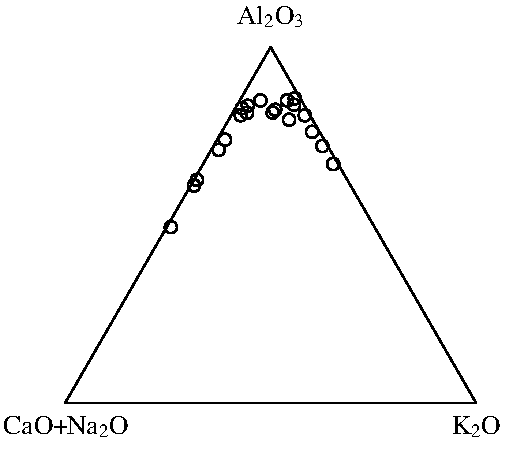
\includegraphics[width=\textwidth]{ACNK.pdf}
  \end{minipage}\hfill
  \begin{minipage}[c]{0.49\textwidth}
    \caption{Graphical output of Section~\ref{sec:compositional}.
      Black circles mark 20 synthetic
      Al\textsubscript{2}O\textsubscript{3}, (CaO +
      Na\textsubscript{2}O) and K\textsubscript{2}O compositions,
      drawn from a logistic normal distribution.  The blue square
      marks the arithmetic mean, which falls outside the data cloud.
      The blue polygon marks a 2-$\sigma$ confidence polygon, which
      plots outside the ternary diagram, in physically impossible
      negative space. The red square represents the geometric mean,
      which firmly plots inside the data cloud. The red confidence
      envelope marks a 95\% confidence region calculated using
      Aitchison's logratio approach. This confidence envelop neatly
      fits inside the ternary diagram and tightly hugs the data.}
    \label{fig:ACNK}
  \end{minipage}
\end{figure}

\section{Point-counting data}
\label{sec:counts}

\textit{\textbf{Summary:} Point-counting data such as heavy mineral
  counts are underlain by compositional distributions. But they are
  not amenable to the logratio transformations introduced in
  Section~\ref{sec:compositional} because they commonly contain zero
  values. Averages and confidence intervals for this type of data
  require hybrid statistical models combining compositional and
  multinomial aspects.}\\

The mineralogical composition of silicilastic sediment can be
determined by tallying the occurrence of various minerals in a
representative sample of (200-400, say) grains \citep{vanderplas1965,
  weltje2002}.  Such \emph{point-counting} data are closely related to
the compositional data that were discussed in the previous
section. However, there are some crucial differences between these two
data classes \citep{vermeesch2018d}.\\

Point-counting data are associated with significant (counting)
uncertainties, which are ignored by classical compositional data
analysis. As a consequence, point-counting data often contain zero
values, which are incompatible with the log-ratio transformation
defined in Equation~\ref{eq:alr}. Although `rounding zeros' also occur
in compositional data, where they can be removed by `imputation'
methods \citep{martin2003, bloemsma2015}, these methods are ill-suited
for point-counting datasets in which zeros are the rule rather than
the exception.

\begin{enumerate}
  
\item Download the auxiliary data file \texttt{HM.csv} from the Online
  Supplement. This file contains a heavy mineral dataset from the
  Namib Sand Sea \citep{vermeesch2015}. It consists of 16 rows (one
  for each sample) and 15 columns (one for each mineral).  Read these
  data into memory and tell \texttt{provenance} to treat it as
  point-counting data in all future operations:

%\begin{tcolorbox}[colback=blue!5!white]
\begin{verbatim}
HM <- read.counts('HM.csv')
\end{verbatim}
%\end{tcolorbox}

\citet{galbraith1988}'s \emph{radial plot} is an effective way to
visually assess the degree to which the random counting uncertainties
account for the observed scatter of binary point-counting
data. Applying this to the epidote/garnet-ratio of the heavy mineral
data (Figure~\ref{fig:radial}):

%\begin{tcolorbox}[colback=blue!5!white]
\begin{verbatim}
radialplot(HM,num='ep',den='gt')
\end{verbatim}
%\end{tcolorbox}

Each circle on the resulting scatter plot represents a single sample
in the \texttt{HM} dataset. Its epidote/garnet-ratio can be obtained
by projecting the circle onto the circular scale. Thus, low and high
ratios are found at negative and positive angles to the origin,
respectively. The horizontal distance of each point from the origin is
proportional to the total number of counts in each sample and, hence,
to its precision. An (asymmetric) 95\% confidence interval for the
ep/gt-ratio of each sample can be obtained by projecting both ends of
a 2-sigma confidence bar onto the circular scale.
\end{enumerate}

Suppose that the data are underlain by a single true population and
random counting uncertainties are the sole source of scatter.  Let
$\theta$ be the true but unknown proportion of the binary
subpopulation that consists of the first mineral (epidote, say). Then
$(1-\theta)$ is the fraction of grains that belong to the second
mineral (garnet).  Further suppose that we have counted a
representative sample of $N$ grains from this population. Then the
probability that this sample contains $n$ grains of the first mineral
and $m=N-n$ grains of the second mineral follows a binomial
distribution:

\begin{equation}
  p(n) = \binom{n+m}{n} \theta^n (1-\theta)^m
  \label{eq:binom}
\end{equation}
  
If multiple samples in a dataset are indeed underlain by the same
fraction $\theta$, then approximately 95\% of the samples should fit
within a horizontal band of two standard errors drawn on either side
of the origin. In this case, $\theta$ can be estimated by
\emph{pooling} all the counts together and computing the proportion of
the first mineral as a fraction of the total number of grains counted
\citep{vermeesch2018d}.\\

However, the ep/gt-ratios in \texttt{HM} scatter significantly beyond
the 2-sigma band (Figure~\ref{fig:radial}.i). The data are therefore
said to be \emph{overdispersed} with respect to the counting
uncertainties. This indicates the presence of true geological
dispersion in the compositions that underly the point-counting data.
The dispersion can be estimated by a \emph{random effects model} with
two parameters:

\begin{equation}
  \beta \equiv \ln\left(\frac{\theta}{1-\theta}\right) \approx
  \mathcal{N}(\mu,\sigma^2)
  \label{eq:central}
\end{equation}

\noindent where $\beta$ is a new variable that follows a normal
distribution with mean $\mu$ and standard deviation $\sigma$, both of
which have geological significance.\\

The `central ratio' is given by $\exp[\hat{\mu}]$ where $\hat{\mu}$ is
the maximum likelihood estimate for $\mu$. This estimates the
geometric mean (\texttt{ep/gt}-) ratio of the true underlying
composition. The `dispersion' ($\hat{\sigma}$) estimates the
geological scatter \citep{galbraith1990a, vermeesch2018d}. In the case
of our heavy mineral dataset, the epidote-garnet subcomposition is
75\% dispersed. This means that the coefficient of variation (standard
deviation divided by geometric mean) of the true epidote/garnet-ratios
is approximately 0.75.

\begin{enumerate}
\setcounter{enumi}{1}
\item The continuous mixtures from the previous section can be
  generalised from two to three or more dimensions. The following code
  snippet uses it to construct a 95\% confidence contour for the
  ternary subcomposition of garnet, epidote and zircon
  (Figure~\ref{fig:radial}.ii).  Note that this dataset contains four
  zero values, which would have rendered the logratio approach of
  Figure~\ref{fig:ACNK} unusable.

%\begin{tcolorbox}[colback=blue!5!white]
\begin{verbatim}
tern <- ternary(HM,x='gt',y='ep',z='zr')
plot(tern,pch=1,labels=NA)
ternary.ellipse(tern,alpha=0.05)
\end{verbatim}
%\end{tcolorbox}

\item For datasets comprising more than three variables, the central
  composition can be simply obtained as follows:

%\begin{tcolorbox}
\begin{verbatim}
> central(HM)
\end{verbatim}
%\end{tcolorbox}
  
This produces a matrix with the proportions of each component; its
standard error; the dispersion of the binary subcomposition formed by
the component and the amalgamation of all remaining components; and
the outcome of a chi-square test for homogeneity.

\end{enumerate}

\begin{figure}[!ht]
  \centering
  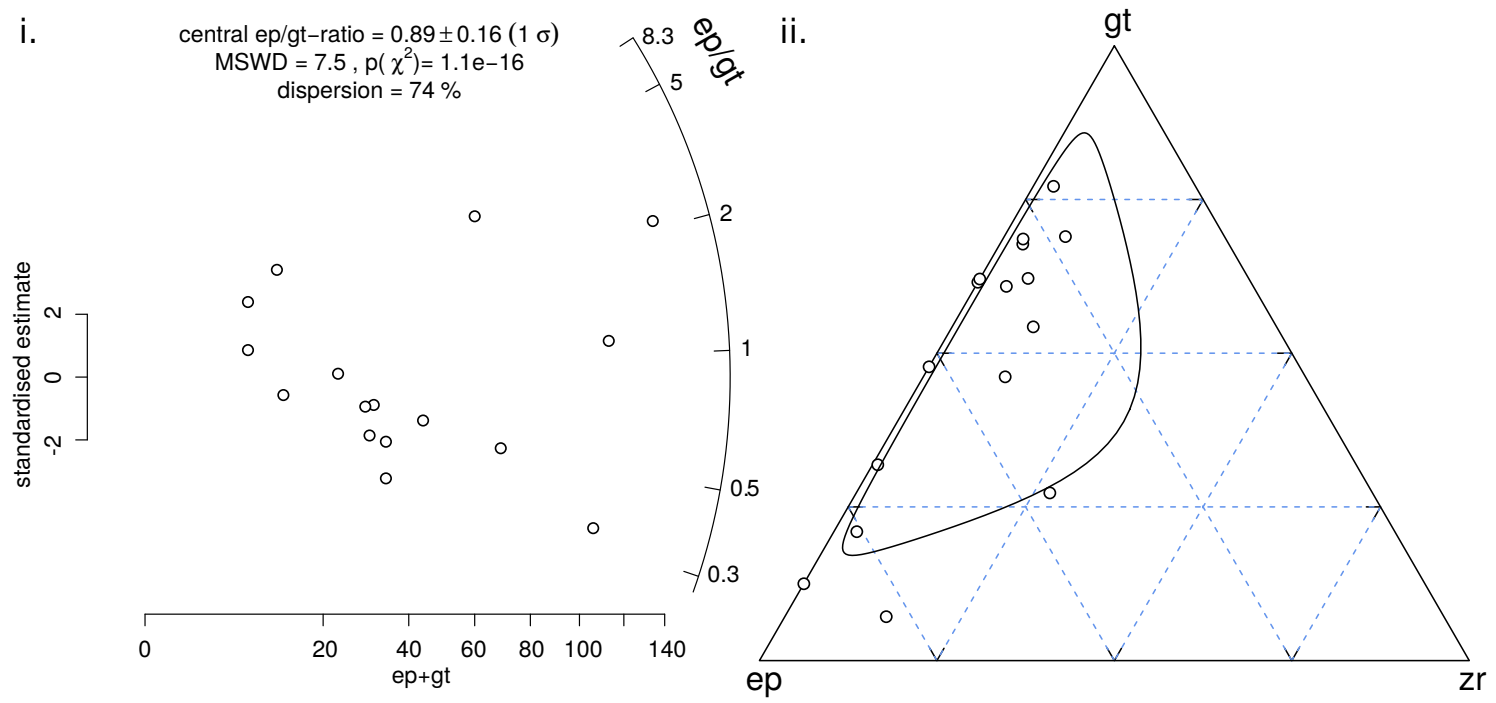
\includegraphics[width=\textwidth]{pointcounts.pdf}
  \caption{i. Radial plot of the epidote/garnet-ratios of 16 samples
    of Namibian desert sand. These data are overdispersed with respect
    to the point-counting uncertainties, indicating 75\% of geological
    scatter in the underlying compositional data. ii. Ternary diagram
    of garnet, epidote and zircon, with a 95\% confidence envelope for
    the underlying population, using a ternary generalisation of the
    random effects model. Note that four of the samples contain zero
    zircon counts. But this does not pose a problem for the random
    effects model, unlike the logratio-procedure used for
    Figure~\ref{fig:ACNK}.}
  \label{fig:radial}
\end{figure}

\section{Distributional data}
\label{sec:distributional}

\textit{\textbf{Summary:} This Section investigates a 16-sample,
  1547-grain dataset of detrital zircon U-Pb ages from Namibia.  It
  uses Kernel Density Estimation and Cumulative Age Distributions to
  visualise this dataset, and introduces the Kolmogorov-Smirnov
  statistic as a means of quantifying the dissimilarity between
  samples.}\\

Compositional data such as the chemical concentrations of
Sections~\ref{sec:compositional} and \ref{sec:compositionalPCA} are
characterised by the relative proportions of a number of
\emph{discrete} \emph{categories}. A second class of provenance
proxies are based on the sampling distribution of \emph{continuous}
variables such as zircon U-Pb ages \citep{fedo2003,
  gehrels2011}. These \emph{distributional} data do not fit in the
statistical framework of the (logistic) normal distribution.

\begin{enumerate}

\item Download auxiliary data file \texttt{DZ.csv} from the Online
  Supplement. This file contains a detrital zircon U-Pb dataset from
  Namibia. It consists of 16 columns --one for each sample-- each
  containing the single grain U-Pb ages of their respective
  sample. Let us load this file into memory using
  \texttt{provenance}'s \texttt{read.distributional} function:

  %\begin{tcolorbox}[colback=blue!5!white]
\begin{verbatim}
DZ <- read.distributional("DZ.csv")
\end{verbatim}
  %\end{tcolorbox}

  \texttt{DZ} now contains an object of class \texttt{distributional}
  containing the zircon U-Pb ages of 16 Namibian sand samples.  To view
  the names of these samples:

  %\begin{tcolorbox}
\begin{verbatim}
> names(DZ)
\end{verbatim}
  %\end{tcolorbox}

\item One way to visualise the U-Pb age distributions is as Kernel Density
  Estimates. A KDE is defined as:

  \begin{equation}
    KDE_x(t) = \frac{1}{n} \sum\limits_{i=1}^{n} \mathcal{K}(t|x_i,bw)
    \label{eq:KDE}
  \end{equation}

  where $\mathcal{K}$ is the `kernel' and $bw$ is the `bandwidth'
  \citep{silverman1986, vermeesch2012b}. The kernel can be any
  unimodal and symmetric shape (such as a box or a triangle), but is
  most often taken to be Gaussian (where $x_i$ is the mean and $bw$
  the standard deviation). The bandwidth can either be set manually,
  or selected automatically based on the number of data points and the
  distance between them. \texttt{provenance} implements the automatic
  bandwidth selection algorithm of \citet{botev2010} but a plethora of
  alternatives are available in the statistics literature. To plot all
  the samples as KDEs:

  %\begin{tcolorbox}[colback=blue!5!white]
\begin{verbatim}
kdes <- KDEs(DZ)
plot(kdes,ncol=2)
\end{verbatim}
  %\end{tcolorbox}

  where \texttt{ncol} specifies the number of columns over which the
  KDEs are divided.

\item Alternatively, the Cumulative Age Distribution (CAD) is a second
  way to show the data \citep{vermeesch2007a}. A CAD is a step
  function that sets out the rank order of the dates against their
  numerical value:

  \begin{equation}
    \mathrm{CAD}(t) = \sum_{i=1}^{n} 1(t<t_i)/n
    \label{eq:CAD}
  \end{equation}

  where $1(\ast) = 1$ if $\ast$ is true and $1(\ast) = 0$ if $\ast$ is
  false. The main advantages of CADs over KDEs is that (i) they do not
  require any smoothing (i.e., there is no `bandwidth' to choose), and
  (ii) they can superimpose multiple samples on the same plot.
  Plotting samples N1, N2 and N4 of the Namib dataset:

  %\begin{tcolorbox}[colback=blue!5!white]
\begin{verbatim}
plot(DZ,snames=c('N1','N2','N4'))
\end{verbatim}
  %\end{tcolorbox}

  we can see that (1) the CADs of samples N1 and N2 plot close
  together with steepest sections at 500~Ma and 1000~Ma, reflecting
  the prominence of those age components; (2) sample N4 is quite
  different from N1 and N2.

\item\label{it:KS} We can quantify this difference using the
  \emph{Kolmogorov-Smirnov} (KS) statistic \citep{feller1948,
    degraaff2003, vermeesch2018b}, which represents the maximum
  vertical difference between two CADs:

  %\begin{tcolorbox}
\begin{verbatim}
> N124 <- subset(DZ,select=c('N1','N2','N4'))
> diss(N124)
\end{verbatim}
  %\end{tcolorbox}

  This shows that the KS-statistic between N1 and N2 is KS(N1,N2) =
  0.18, whereas KS(N1,N4) = 0.44, and KS(N2,N4) = 0.35
  (Figure~\ref{fig:CADs}). The KS statistic is a \emph{non-negative}
  value that takes on values between zero (perfect overlap between two
  distributions) and one (no overlap between two distributions). It is
  \emph{symmetric} because the KS statistic between any sample $x$ and
  another sample $y$ equals that between $y$ and $x$. For example,
  KS(N1,N2) = 0.18 = KS(N2,N1).  And finally, the KS-statistic obeys
  the \emph{triangle equality}, which means that the dissimilarity
  between any two samples is always smaller than or equal to the sum
  of the dissimilarities between those two samples and a third.  For
  example, KS(N1,N2) = 0.18 $<$ KS(N1,N4) + KS(N2,N4) = 0.44 + 0.35 =
  0.79. These three characteristics qualify the KS statistics as a
  \emph{metric}, which makes it particularly suitable for
  Multidimensional Scaling (MDS) analysis (see Section~\ref{sec:MDS}).
  The KS statistic is just one of many dissimilarity measures for
  distributional data.  However, not all these alternatives to the KS
  statistic fulfil the triangle inequality \citep{vermeesch2018b}.

\end{enumerate}

\begin{figure}[!ht]
  \begin{minipage}[c]{0.69\textwidth}
    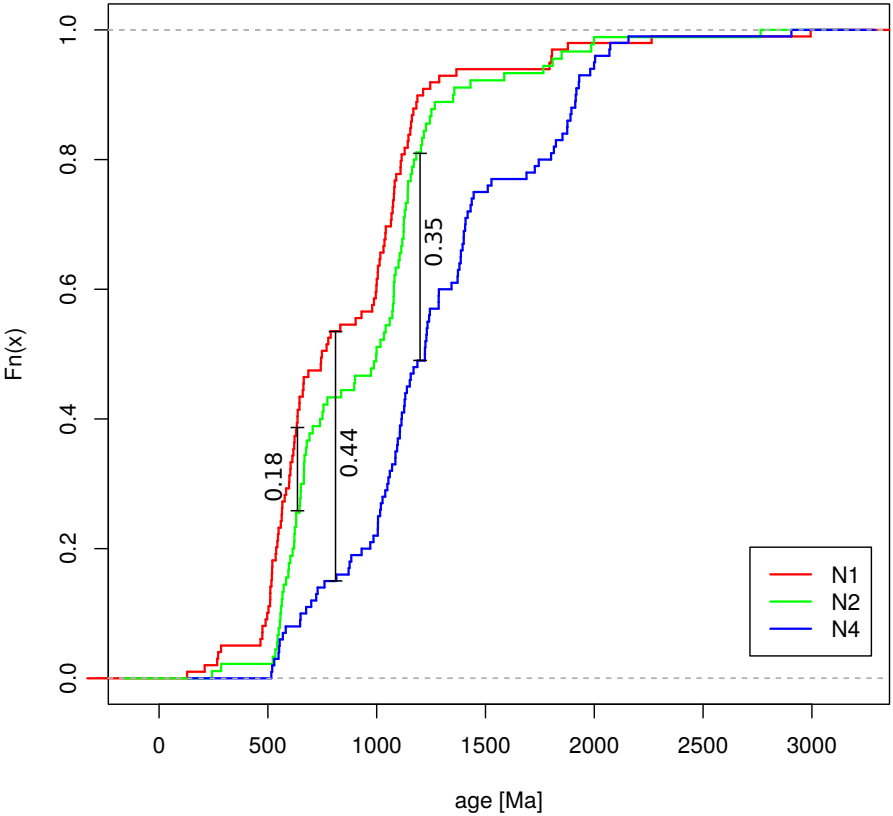
\includegraphics[width=\textwidth]{CADs.pdf}
  \end{minipage}\hfill
  \begin{minipage}[c]{0.30\textwidth}
    \caption{
      Cumulative Age Distributions (CADs) of Namib desert sand
      samples N1, N2 and N4 with indication of the Kolmogorov-Smirnov
      distances between them.
    } \label{fig:CADs}
  \end{minipage}
\end{figure}


\section{Principal Component Analysis (PCA)}
\label{sec:PCA}

\textit{\textbf{Summary:} Principal Component Analysis is an
  exploratory data analysis method that takes a high dimensional
  dataset as input and produces a lower (typically two-) dimensional
  `projection' as output. PCA is closely related to Multidimensional
  Scaling (MDS), compositional PCA, and Correspondence Analysis (CA),
  which are introduced in Sections~\ref{sec:MDS}--\ref{sec:CA}. This
  tutorial introduces PCA using the simplest working example of three
  two-dimensional points. Nearly identical examples will be used in
  Sections~\ref{sec:MDS}--\ref{sec:CA}.}

\begin{enumerate}
\item
  Consider the following bivariate ($a$ and $b$) dataset of three (1, 2
  and 3) samples:

  \begin{equation}
    X = \bbordermatrix{ & a & b \cr
      1 & -1 & 7 \cr
      2 & 3 & 2 \cr
      3 & 4 & 3
    }
    \label{eq:X}
  \end{equation}

  Generating and plotting $X$ in \texttt{R}:

  %\begin{tcolorbox}[colback=blue!5!white]
\begin{verbatim}
X <- matrix(c(-1,3,4,7,2,3),nrow=3,ncol=2)
colnames(X) <- c('a','b')
plot(X)
\end{verbatim}
  %\end{tcolorbox}

  \noindent yields a diagram in which two of the three data points
  plot close together while the third one plots further away.

\item Imagine that you live in a one-dimensional world and cannot see
  the spatial distribution of the three points represented by
  $X$. Principal Component Analysis (PCA) is a statistical technique
  \citep[invented by Karl][]{pearson1901} to represent multi- (e.g.,
  two-) dimensional data in a lower- (e.g., one-) dimensional space
  whilst preserving the maximum amount of information (i.e.,
  variance). This can be achieved by decomposing $X$ into four
  matrices ($C$, $S$, $V$ and $D$):

  \begin{equation}
      X = ~ 1_{3,1}~C + S~V~D =
        \left[
        \begin{array}{c}
          1 \\
          1 \\
          1
        \end{array}
        \right]
      \left[
        \begin{array}{cc}
          2 & 4
        \end{array}
        \right]
      +
      \left[
        \begin{array}{cc}
          -1.15 & 0 \\
          0.58 & -1 \\
          0.58 & 1
        \end{array}
        \right]
      \left[
        \begin{array}{cc}
          3.67 & 0 \\
          0 & 0.71
        \end{array}
        \right]
      \left[
        \begin{array}{cc}
          0.71 & -0.71\\
          0.71 & 0.71
        \end{array}
        \right]
      \label{eq:PCA}
  \end{equation}

  \noindent where $C$ is the centre (arithmetic mean) of the two data
  columns; $S$ are the \emph{normalised scores}; the diagonals of $V$
  correspond to the standard deviations of the two principal components;
  and $D$ is a rotation matrix (the \emph{principal directions}). $S$,
  $V$ and $D$ can be recombined to define two more matrices:

  \begin{equation}
    P  = S~V =
    \left[
      \begin{array}{cc}
        -4.24 & 0 \\
        2.12 & -0.71 \\
        2.12 & 0.71
      \end{array}
      \right] \mbox{, and}\label{eq:P}
  \end{equation}\\
  
  \begin{equation} L = V~D  =
    \left[
      \begin{array}{cc}
        2.6 & -2.6 \\
        0.5 & 0.5 \\
      \end{array}
      \right]
    \label{eq:L}
  \end{equation}

  \noindent where $P$ is a matrix of transformed coordinates (the
  \emph{principal components} or \emph{scores}) and $L$ are the scaled
  eigenvectors or \emph{loadings}. Figure~\ref{fig:PCA}.i shows $X$ as
  numbers on a scatterplot, $C$ as a yellow square, and $1_{2,1}C \pm
  L$ as a cross. Thus, the first principal direction (running from the
  upper left to the lower right) has been stretched by a factor of
  $(3.67/0.71) = 5.2$ w.r.t the second principal component, which runs
  perpendicular to it. The two principal components are shown
  separately as Figure~\ref{fig:PCA}.ii, and their relative
  contribution to the total variance of the data as
  Figure~\ref{fig:PCA}.iv. Figure~\ref{fig:PCA} can be reproduced with
  the following \texttt{R}-code:

  %\begin{tcolorbox}[colback=blue!5!white]
\begin{verbatim}
source('helper.R')
PCA2D(X)
\end{verbatim}
  %\end{tcolorbox}

\item Although the two-dimensional example is useful for illustrative
  purposes, the true value of PCA obviously lies in higher dimensional
  situations. As a second example, let us consider one of \texttt{R}'s
  built-in datasets. \texttt{USArrests} contains statistics (in
  arrests per 100,000 residents) for assault, murder, and rape in each
  of the 50 US states in 1973. Also given is the percentage of the
  population living in urban areas. Thus, \texttt{USArrests} is a
  four-column table that cannot readily be visualised on a
  two-dimensional surface. Applying PCA yields four principal
  components, the first two of which represent 62\% and 25\% of the
  total variance, respectively. Because the four columns of the input
  data are expressed in different units (arrests per 100,000 or
  percentage), it is necessary to scale the data to have unit variance
  before the analysis takes place:

  %\begin{tcolorbox}[colback=blue!5!white]
\begin{verbatim}
pc <- prcomp(USArrests, scale=TRUE) 
biplot(pc)
\end{verbatim}
  %\end{tcolorbox}

  You will see that the loading vectors for \texttt{Murder},
  \texttt{Assault} and \texttt{Rape} are all pointing in approximately
  the same direction (dominating the first principal component),
  perpendicular to \texttt{UrbanPop} (which dominates the second
  principal component). This tells us that crime and degree of
  urbanisation are not correlated in the United States.

\end{enumerate}

\begin{figure}[!ht]
  \centering
  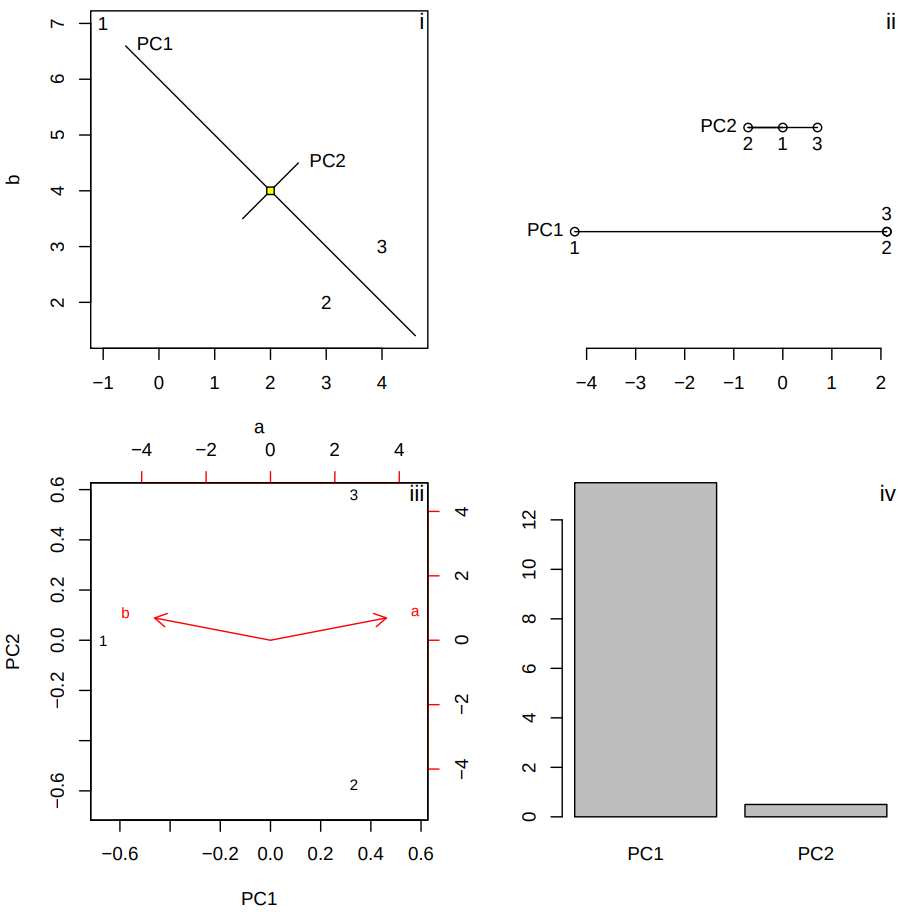
\includegraphics[width=.8\textwidth]{PCA.pdf}
  \caption{i -- Three samples (1, 2 and 3) of bivariate ($a$ and $b$)
    data ($X$ in Equation~\ref{eq:X}). The yellow square marks the
    arithmetic mean ($C$ in Equation~\ref{eq:PCA}), the cross marks
    the two principal directions ($D$ in Equation~\ref{eq:PCA})
    stretched by the diagonal elements (i.e. the standard deviations)
    of $V$ (Equation~\ref{eq:PCA}); ii -- The projection of the data
    points on these two directions yields two principal components
    ($P$ in Equation~\ref{eq:P}), representing a one dimensional
    representation of the two-dimensional data; iii -- A biplot of
    both principal components along with the loadings of the two
    variables shown as arrows; iv -- The squared diagonal values of
    $V$ (Equation~\ref{eq:PCA}) indicate the relative amounts of
    variance encoded by the two principal components.}
  \label{fig:PCA}
\end{figure}

\section{Multidimensional Scaling}
\label{sec:MDS}

\textit{\textbf{Summary:} Multidimensional Scaling (MDS) is a less
  restrictive superset of PCA. This tutorial uses a geographical
  example to demonstrate how MDS re-creates a map of Europe from a
  table of pairwise distances between European cities. Applying the
  same algorithm to the synthetic toy-example of Section~\ref{sec:PCA}
  yields exactly the same output as PCA.}

\begin{enumerate}

\item Multidimensional Scaling \citep[MDS,][]{young1938,
  torgerson1952, shepard1962, kruskal1978} is a dimension-reducing
  technique that aims to extract two (or higher) dimensional `maps'
  from tables of pairwise distances between objects. This method is
  most easily illustrated with a geographical example. Consider, for
  example, the \texttt{eurodist} dataset that is built into
  \texttt{R}, and which gives the road distances (in km) between 21
  cities in Europe (see \texttt{?eurodist} for further details):

  %\begin{tcolorbox}
\begin{verbatim}
> eurodist
\end{verbatim}
  %\end{tcolorbox}

\item To MDS configuration can be obtained by \texttt{R}'s built-in
  \texttt{cmdscale} function
  
  %\begin{tcolorbox}[colback=blue!5!white]
\begin{verbatim}
conf <- cmdscale(eurodist)
\end{verbatim}
  %\end{tcolorbox}

Set up an empty plot with a 1:1 aspect ratio, and then label the MDS
configuration with the city names:

  %\begin{tcolorbox}[colback=blue!5!white]
\begin{verbatim}
plot(conf,type='n',asp=1)
text(conf,labels=labels(eurodist))
\end{verbatim}
  %\end{tcolorbox}

  Note that the map may be turned `upside down'. This reflects the
  rotation invariance of MDS configurations.

\item \texttt{R}'s \texttt{cmdscale} function implements so-called
  `classical' MDS, which aims to fit the actual distances
  \citep{young1938, torgerson1952}. If these distances are Euclidean,
  then it can be shown that MDS is equivalent to PCA
  \citep{aitchison1983, kenkel1986, cox2000}. To demonstrate this
  equivalence, let us apply MDS to the data in Equation~\ref{eq:X}.
  First run the first two lines of code from
  Section~\ref{sec:PCA}. Calculating the Euclidean distances between
  the three samples produces a dissimilarity matrix $d$.  For example,
  the distance between points 1 and 2 is $\sqrt{(-1-3)^2+(7-2)^2} =
  6.4$.  This value is stored in \texttt{d[1,1]}. In \texttt{R}:

  %\begin{tcolorbox}[colback=blue!5!white]
\begin{verbatim}
d <- dist(X)
\end{verbatim}
  %\end{tcolorbox}

  which produces:

  \begin{equation}
    d =
    \bbordermatrix{ & 1 & 2 & 3\cr
      1 & 0 & 6.4 & 6.4 \cr
      2 & 6.4 & 0 & 1.4 \cr 
      3 & 6.4 & 1.4 & 0
    }
    \label{eq:d}
  \end{equation}

\item Next, calculate the MDS configuration:
  
  %\begin{tcolorbox}[colback=blue!5!white]
\begin{verbatim}
conf2 <- cmdscale(d)
\end{verbatim}
  %\end{tcolorbox}

  Finally, plot the MDS configuration as a scatterplot of text labels:

  %\begin{tcolorbox}[colback=blue!5!white]
\begin{verbatim}  
plot(conf2,type='n')
text(conf2,labels=1:3)
\end{verbatim}
  %\end{tcolorbox}

Which is identical to the PCA configuration of
Figure~\ref{fig:PCA}.iii apart from an arbitrary rotation or
reflection.

\item\label{it:nonmetricMDS} An alternative implementation of MDS
  loosens the Euclidean distance assumption by fitting the
  \emph{relative} distances between objects \citep{shepard1962,
    kruskal1978}. Let us apply this to the dataset of European city
  distances using the \texttt{isoMDS} function of the `Modern Applied
  Statistics with S' (\texttt{MASS}) package \citep{ripley2002}:

  %\begin{tcolorbox}[colback=blue!5!white]
\begin{verbatim}
library(MASS)
\end{verbatim}
  %\end{tcolorbox}

To compute and plot the non-metric MDS configuration:
  
  %\begin{tcolorbox}[colback=blue!5!white]
\begin{verbatim}
conf3 <- isoMDS(eurodist)$points
plot(conf3,type='n',asp=1)
text(conf3,labels=labels(eurodist))
\end{verbatim}
  %\end{tcolorbox}

  where \texttt{conf3} is a list with two items: \texttt{stress},
  which expresses the goodness-of-fit of the MDS configuration; and
  \texttt{points}, which contains the configuration. The `\texttt{\$}'
  operator is used to access any of these items.\\
  
  Non-metric MDS is a less-restrictive superset of classical MDS and,
  hence, PCA, which opens this methodology up to non-Euclidean
  dissimilarity measures, such as the KS-distance introduced in
  Section~\ref{sec:distributional} \citep{vermeesch2013}.

\end{enumerate}

\section{PCA of compositional data}
\label{sec:compositionalPCA}

\textit{\textbf{Summary:} PCA can be applied to compositional data
  after logratio transformation. This tutorial first applies such
  compositional PCA to a three sample, three variable dataset that is
  mathematically equivalent to the three sample two variable toy
  example of Section~\ref{sec:PCA}. Then, it applies the same method
  to a real dataset of major element compositions from Namibia. This
  is first done using basic \textnormal{\texttt{R}} and then again
  (and more succinctly) using the \textnormal{\texttt{provenance}}
  package.}\\

Consider the following trivariate ($a$, $b$ and $c$) dataset of three
(1, 2 and 3) compositions:

\begin{equation}
  X =
  \bbordermatrix{ & a & b & c \cr
   1 & 0.03 & 99.88 & 0.09 \cr
   2 & 70.54 & 25.95 & 3.51 \cr
   3 & 72.14 & 26.54 & 1.32
  }
  \label{eq:Xcomp}
\end{equation}

It would be wrong to apply conventional PCA to this dataset, because
this would ignore the constant sum constraint.  As was discussed in
Section~\ref{sec:PCA}, PCA begins by `centering' the data via the
arithmetic mean. Section~\ref{sec:compositional} showed that this
yields incorrect results for compositional data. Subjecting the data
to a logratio transformation produces:

\begin{equation}
  X\textsubscript{a} =
  \bbordermatrix{ & \ln(a/c) & \ln(b/c) \cr
    1 & -1 & 7 \cr
    2 & 3 & 2 \cr
    3 & 4 & 3
  }
  \label{eq:Xa}
\end{equation}

\noindent which, the observant reader will note, is identical to the
example of Equation~\ref{eq:X}. Applying conventional PCA to the
log-transformed data of Equation~\ref{eq:Xa} will yield two principal
components that are expressed in terms of the logratios ln($a/c$) and
ln($b/c$).\\

Alternatively, the data of Equation~\ref{eq:Xcomp} can also be
subjected to a different type of logratio transformation
\citep{aitchison1983}. The so-called \emph{centred} logratio
transformation (as opposed to the \emph{additive} logratio
transformation of Equation~\ref{eq:alr} maps any set of compositional
data vectors $x = \{x_1, \dots, x_i, \dots, x_n\}$, $y = \{y_1, \dots,
y_i, \dots, y_n\}$, ... to the same number of (centred) logratios $u =
\{u_1, \dots, u_i, \dots, u_n\}$, $v = \{v_1, \dots, v_i, \dots,
v_n\}$, ..., where:

\begin{equation}
  u_i = \ln(x_i) - [\ln(x_i)+\ln(y_i)]/2
  \mbox{~and~}
  v_i = \ln(y_i) - [\ln(x_i)+\ln(y_i)]/2
  \label{eq:clr}
\end{equation}

Applying this transformation to the data of Equation~\ref{eq:Xcomp}
yields a new trivariate dataset:

\begin{equation}
  X\textsubscript{c} =
  \bbordermatrix{ & \ln(a/g) & \ln(b/g) & \ln(c/g) \cr
    1 & -3 & 5 & -2 \cr
    2 & 1.33  & 0.33 & -1.67 \cr
    3 & 1.67  & 0.67 & -2.33
  }
  \label{eq:Xc}
\end{equation}

\noindent where $g$ stands for the geometric mean of each
row. Subjecting Equation~\ref{eq:Xc} to the same matrix decomposition
as Equation~\ref{eq:PCA} yields:
  
\begin{equation}
    X_c = 1_{3,1}~C + S~V~D = \left[
      \begin{array}{c}
        1 \\
        1 \\
       1
      \end{array}
      \right]
   \left[
    \begin{array}{ccc}
        0 & 2 & -2
      \end{array}
      \right]
    + 
    \left[
      \begin{array}{ccc}
        -1.15 &  0 & 0.82 \\
        0.58  & -1 & 0.82 \\
        0.58  &  1 & 0.82
      \end{array}
      \right]
    \left[
      \begin{array}{ccc}
        3.67 & 0 & 0 \\
        0 & 0.41 & 0 \\
        0 & 0 & 0
      \end{array}
      \right]
    \left[
      \begin{array}{ccc}
        0.71 & -0.71 &  0 \\
        0.41 &  0.41 & -0.82 \\
        0.58 &  0.58 &  0.58
      \end{array}
      \right]
    \label{eq:PCAcomp}
  \end{equation}

Note that, even though this yields three principal components instead
two, the standard deviation of the third component is zero.
Therefore, all the information is contained in the first two
components.  The PCA map using the centred logratio transformation
looks identical to that using the additive logratio
transformation. The only difference is that the loadings are expressed
in terms of the three centred logratio variables, rather than the two
additive logratio variables. The centred logratios are easier to
interpret than the additive logratios, which is why the centred
logratio transformation is preferred in this context.

\begin{figure}[!ht]
  \centering
  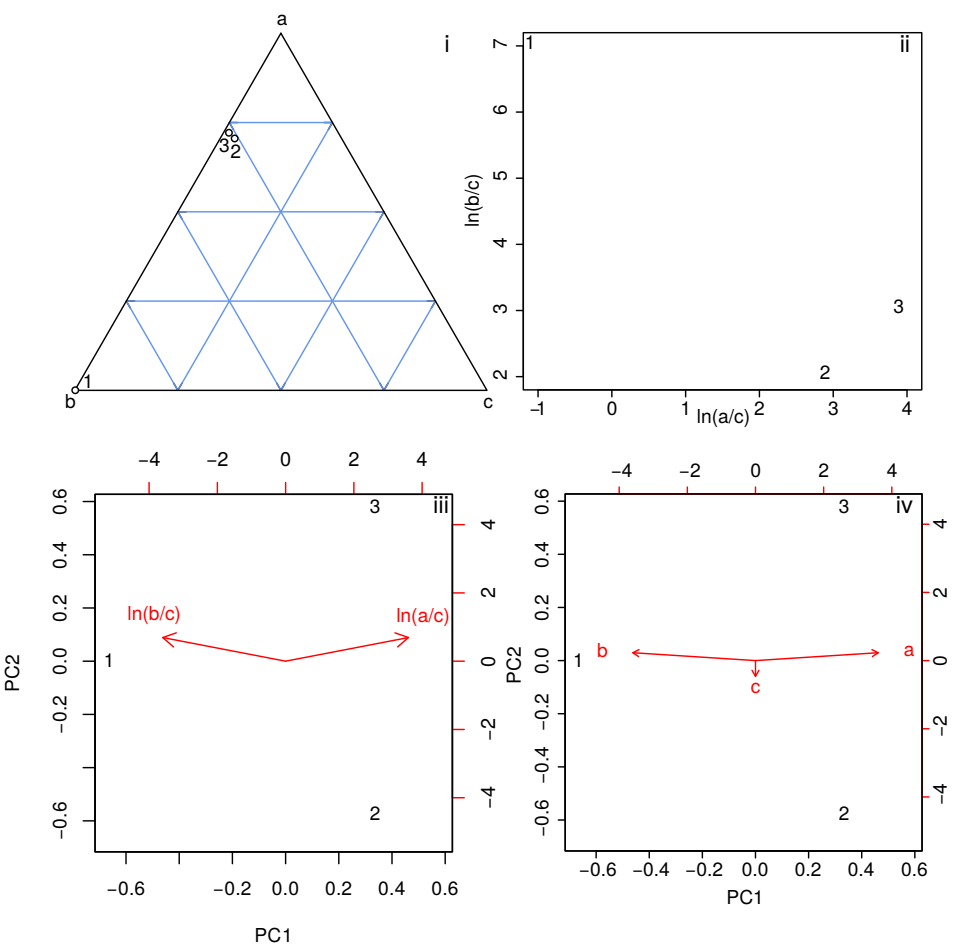
\includegraphics[width=.8\textwidth]{compositionalPCA.pdf}
  \caption{i -- the compositional dataset of Equation~\ref{eq:Xc}
    shown on a ternary diagram; ii -- subjecting the same dataset to
    an additive logratio transformation (alr) produces a configuration
    of points that is identical to Figure~\ref{fig:PCA}.i; iii --- as
    a consequence the PCA biplot of the logratio transformed data
    looks identical to Figure~\ref{fig:PCA}.iii; iv -- using a centred
    logratio transformation (clr) yields the same configuration as
    panel iii but with more easily interpretable vector loadings.}
  \label{fig:compositionalPCA}
\end{figure}

\begin{enumerate}
  \item The following script applies compositional PCA to a dataset of
    major element compositions from Namibia (see Online Supplement)
    using base \texttt{R}:

  %\begin{tcolorbox}[colback=blue!5!white]
\begin{verbatim}
# load the major element composition of Namib sand:
Major <- read.csv(file="Major.csv",
                  header=TRUE,row.names=1)
# apply the centred logratio transformation:
cMajor <- log(Major) - 
       rowMeans(log(Major)) %*% matrix(1,1,ncol(Major))
# perform PCA of the logratio transformed data:
pc <- prcomp(cMajor)
# plot the results of the PCA analysis:
biplot(pc)
\end{verbatim}
  %\end{tcolorbox}

\item Alternatively, we can also do this more easily in
  \texttt{provenance}:

  %\begin{tcolorbox}[colback=blue!5!white]
\begin{verbatim}
library(provenance)
# tell R that Major.csv contains compositional data:
Major.comp <- read.compositional('Major.csv')
# perform the principal component analysis:
pc.comp <- PCA(Major.comp)
# create the biplot:
plot(pc.comp)
\end{verbatim}
  %\end{tcolorbox}

  where the \texttt{read.compositional} function reads the
  \texttt{.csv} file into an object of class \texttt{compositional},
  thus ensuring that logratio statistics are used in all
  \texttt{provenance} functions (such as \texttt{PCA}) that accept
  compositional data as input. Also note that the \texttt{provenance}
  package \emph{overloads} the \texttt{plot} function to generate a
  compositional biplot when applied to the output of the \texttt{PCA}
  function.

\end{enumerate}

\section{Correspondence Analysis}
\label{sec:CA}

\textit{\textbf{Summary:} Point-counting data can be analysed by MDS
  using the Chi-square distance. Correspondence Analysis (CA) yields
  identical results whilst producing biplots akin to those obtained by
  PCA. This tutorial first uses a simple three sample, three variable
  toy example that is (almost) identical to those used in
  Sections~\ref{sec:PCA}-\ref{sec:compositionalPCA}, before applying
  CA to a real dataset of heavy mineral counts from Namibia.}\\

Consider the following three sets of trivariate point-counting data:

\begin{equation}
  X = \bbordermatrix{ & a & b & c \cr 1 & 0 & 100 & 0 \cr 2 & 38 &
    13 & 1 \cr 3 & 108 & 38 & 0 }
  \label{eq:Xcounts}
\end{equation}

This dataset intentionally looks similar on a ternary diagram to the
compositional dataset of Section~\ref{sec:compositional}.  The only
difference is the presence of zeros, which preclude the use of
logratio statistics. This problem can be solved by replacing the zero
values with small numbers, but this only works when their number is
small \citep{martin2003, bloemsma2015}. Correspondence Analysis (CA)
is an alternative approach that does not require such `imputation'.\\

CA is a dimension reduction technique that is similar in many ways to
PCA \citep{greenacre1984, vermeesch2018d}. CA, like PCA, is a special
case of MDS. Whereas ordinary PCA uses the Euclidean distance, and
compositional data can be compared using the Aitchison distance,
point-counting data can be compared by means of a chi-square distance:

\begin{equation}
  d_{ij} =
  \sqrt{
    \sum\limits_{k=1}^K
    \frac{X_{\cdot\cdot}}{X_{\cdot k}}
    \left(\frac{X_{ik}}{X_{i\cdot}} - \frac{X_{jk}}{X_{j \cdot}}\right)^2
  }
  \label{eq:dij}
\end{equation}

\noindent where $X_{\cdot k} = \sum_{i=1}^{m}X_{ik}$, $X_{i\cdot} =
\sum_{k=1}^{K}X_{ik}$ and $X_{\cdot\cdot} =
\sum_{i=1}^{m}\sum_{k=1}^{K}X_{ik}$. Applying this formula to the data
of Equation~\ref{eq:Xcounts} produces the following dissimilarity
matrix:

\begin{equation}
  \bbordermatrix{ & 1 & 2 & 3\cr
    1 & 0 & 1.5 & 1.5 \cr
    2 & 1.5 & 0 & 0.33 \cr 
    3 & 1.5 & 0.33 & 0
  }
  \label{eq:dcounts}
\end{equation}

Note that, although these values are different than those in
Equation~\ref{eq:d}, the ratios between them are (approximately) the
same. Specifically, $d_{1,2}/d_{1,3} = 1.5/1.5 = 1$ for
Equation~\ref{eq:dcounts} and $d_{1,2}/d_{1,3} = 6.4/6.4 = 1$ for
Equation~\ref{eq:d}; or $d_{1,2}/d_{2,3} = 1.5/0.33 = 4.5$ for
Equation~\ref{eq:dcounts} and $d_{1,2}/d_{2,3} = 6.4/1.4 = 4.5$ for
Equation~\ref{eq:d}.  Therefore, when we subject our point-counting
data to an MDS analysis using the chi-square distance, the resulting
configuration appears nearly identical to the example of
Section~\ref{sec:MDS}.\\

The following script applies CA to the heavy mineral composition of
Namib desert sand. It loads a table called \texttt{HM.csv} that
contains point counts for 16 samples and 15 minerals.  To reduce the
dominance of the least abundant components, the code extracts the most
abundant minerals (epidote, garnet, amphibole and clinopyroxene) from
the datasets and amalgamates the ultra-stable minerals (zircon,
tourmaline and ru- tile), which have similar petrological
significance.

%\begin{tcolorbox}[colback=blue!5!white]
\begin{verbatim}
library(provenance)
# tell R that HM.csv contains point-counting data:
dat <- read.counts('HM.csv')
# select and amalgamate the components of interest:
HM <- amalgamate(dat,ztr=c('zr','tm','rt'),ep='ep',
                     gt='gt',amp='amp',cpx='cpx')
# perform the correspondence analysis:
config <- CA(HM)
# plot the results as a biplot:
plot(config)
\end{verbatim}
%\end{tcolorbox}

\section{MDS analysis of distributional data}
\label{sec:DZMDS}

\textit{\textbf{Summary:} This brief tutorial applies MDS to the
  detrital zircon U-Pb dataset from Namibia, using the
  Kolmogorov-Smirnov statistic as a dissimilarity measure.}\\

Section~\ref{sec:MDS}.\ref{it:nonmetricMDS} introduced non-metric MDS
as a less-restrictive superset of classical MDS and, hence, PCA. This
opens this methodology up to non-Euclidean dissimilarity measures,
such as the KS-distance introduced in
Section~\ref{sec:distributional}.\ref{it:KS} \citep{vermeesch2013,
  vermeesch2018b}.

%\begin{tcolorbox}[colback=blue!5!white]
\begin{verbatim}
library(provenance)
# read the detrital zircon dataset:
DZ <- read.distributional("DZ.csv")
# calculate and plot the (non-metric)
# MDS configuration using the KS distance:
DZ.X <- MDS(DZ)
plot(DZ.X)
\end{verbatim}
%\end{tcolorbox}

In this case, the overloaded \texttt{plot} function produces not one
but two graphics windows. The first of these shows the MDS
configuration, whereas the second shows the \emph{Shepard plot}
\citep{shepard1962, kruskal1978}. This is a scatterplot that sets out
the Euclidean distances between the samples measured on the MDS
configuration against the \emph{disparities}, which are defined as:

\begin{equation}
  \delta[i,j] = f(KS[i,j])
\end{equation}

where $KS[x_i,x_j]$ is the KS-distance between the
$i$\textsuperscript{th} and $j$\textsuperscript{th} sample and $f$ is
a monotonic transformation, which is shown as a step-function.  The
Shepard plot allows the user to visually assess the goodness-of-fit of
the MDS configuration. This can be further quantified using the
`stress' parameter:

\begin{equation}
  S = \sum_i\sum_j(d[i,j]-\delta[i,j])^2\bigg/\sum_i\sum_j(d[i,j])^2
\end{equation}

The lower the stress, the better the fit. For moderately sized
datasets, stress values should be less than 10\%
\citep{kruskal1978}. For larger datasets, a higher dimensional
solution may be necessary, using the optional parameter \texttt{k} of
\texttt{provenance}'s \texttt{MDS} function \citep{stephan2018}.
  
\section{`Big' data}
\label{sec:bigdata}

\textit{\textbf{Summary:} The tutorial jointly analyses 16 Namibian
  samples using five different provenance proxies, including all three
  data classes introduced in
  Sections~\ref{sec:compositional}-\ref{sec:distributional}. It
  introduces Procrustes Analysis and 3-way MDS as two alternative ways
  to extract geologically meaningful information from these
  multivariate `big' dataset.}\\

It is increasingly common for provenance studies to combine
compositional, point-counting or distributional datasets together
\citep{vermeesch2015, rittner2016}.  Linking together bulk sediment
data, heavy mineral data and single mineral data requires not only a
sensible statistical approach, but also a full appraisal of the impact
of mineral fertility and heavy mineral concentration in eroded bedrock
and derived clast sediment \citep{garzanti2007, malusa2016,
  malusa2019b}. Assuming that this appraisal has been made, this
Section introduces some exploratory data analysis tools that can
reveal meaningful structure in complex datasets.

\begin{enumerate}

\item The full Namib Sand Sea study that we have used as a test case
  for this tutorial comprises no fewer than five datasets (see Online
  Supplement):

  \begin{enumerate}
  \item Major element concentrations (\texttt{Major.csv}, compositional data)
  \item Trace element concentrations (\texttt{Trace.csv}, compositional data)
  \item Bulk petrography (\texttt{PT.csv}, point-counting data)
  \item Heavy mineral compositions (\texttt{HM.csv}, point-counting data)
  \item Detrital zircon U-Pb data (\texttt{DZ.csv}, distributional data)
  \end{enumerate}

  All these datasets can be visualised together in a single summary
  plot:

  %\begin{tcolorbox}[colback=blue!5!white]
\begin{verbatim}
library(provenance)
# major elements:
Major <- read.compositional('Major.csv')
# trace elements:
Trace <- read.compositional('Trace.csv')
# petrography:
QFL <- read.counts('PT.csv',colmap=cm.colors)
# heavy minerals:
HM <- read.counts('HM.csv',colmap=cm.colors)
# zircon U-Pb dates:
DZ <- read.distributional('DZ.csv')
# generate the plot:
summaryplot(Major,Trace,QFL,HM,KDEs(DZ),ncol=2)
\end{verbatim}
  %\end{tcolorbox}

  where \texttt{Major}, \texttt{Trace}, \texttt{QFL} and \texttt{HM}
  are shown as pie charts (the latter two with a different colour map
  than the former), and \texttt{DZ} as KDEs. Adding \texttt{DZ}
  instead of \texttt{KDEs(DZ)} would plot the U-Pb age distributions
  as histograms.

\item The entire Namib dataset comprises 16,125 measurements spanning
  five dimensions worth of compositional, distributional and
  point-counting information.  This complex dataset, which may be
  rightfully described by the internet-era term of `Big Data', is
  extremely difficult to interpret by mere visual inspection of the
  pie charts and KDEs.  Applying MDS/PCA to each of the five
  individual datasets helps but presents the analyst with a multi-plot
  comparison problem. \texttt{provenance} implements two methods to
  address this issue \citep{vermeesch2015}. The first of these is
  called `Procrustes Analysis' \citep{gower1975}. Given a number of
  MDS configurations, this technique uses a combination of
  transformations (translation, rotation, scaling and reflection) to
  extract a `consensus view' for all the data considered together:

  %\begin{tcolorbox}[colback=blue!5!white]
\begin{verbatim}
proc <- procrustes(Major,Trace,QFL,HM,DZ)
plot(proc)
\end{verbatim}
  %\end{tcolorbox}

\item Alternatively, `3-way MDS' is an extension of `ordinary' (2-way)
  MDS that accepts 3-dimensional dissimilarity matrices as
  input. \texttt{provenance} includes the most common implementation
  of this class of algorithms, which is known as `INdividual
  Difference SCALing' or INDSCAL \citep{carroll1970, deleeuw2009}:

  %\begin{tcolorbox}[colback=blue!5!white]
\begin{verbatim}
scal <- indscal(Major,Trace,QFL,HM,DZ)
plot(scal)
\end{verbatim}
  %\end{tcolorbox}

This code produces two pieces of graphical output
(Figure~\ref{fig:INDSCAL}). The `group configuration' represents the
consensus view of all provenance proxies considered together.  This
looks very similar to the Procrustes configuration created by the
previous code snippet. The second piece of graphical information
displays not the samples but the provenance proxies. It shows the
weights that each of the proxies attach to the horizontal and vertical
axis of the group configuration.\\

For example, the heavy mineral compositions of the Namib desert sands
can be (approximately) described by stretching the group configuration
vertically by a factor of 1.9, whilst shrinking it horizontally by a
factor of 0.4. In contrast, the configurations of the major and trace
element compositions for the same samples are obtained by shrinking
the group configuration vertically by a factor 0.8, and stretching it
horizontally by a factor of 1.3. Thus, by combining these weights with
the group configuration yields five `private spaces' that aim to fit
each of the individual datasets.\\

INDSCAL group configurations are not rotation-invariant, in contrast
with the 2-way MDS configurations of Section~\ref{sec:MDS}. This gives
geological meaning to the horizontal and vertical axes of the plot.
For example, samples N1 and N10 plot along a vertical line on the
group configuration, indicating that they have different heavy mineral
compositions, but similar major and trace element compositions.  On
the other hand, samples N4 and N8 plot along a horizontal line,
indicating that they have similar major and trace element compositions
but contrasting heavy mineral compositions.\\

Closer inspection of the weights reveals that the datasets obtained
from fractions of specific densities (\texttt{HM}, \texttt{PT} and
\texttt{DZ}) attach stronger weights to the vertical axis, whereas
those that are determined on bulk sediment (\texttt{Major} and
\texttt{Trace}) dominate the horizontal direction. Provenance proxies
that use bulk sediment are more sensitive to winnowing effects than
those that are based on density separates. This leads to the
interpretation that the horizontal axis separates samples that have
been affected by different degrees of hydraulic sorting, whereas the
vertical direction separates samples that have different provenance.

\end{enumerate}

\begin{figure}[!ht]
  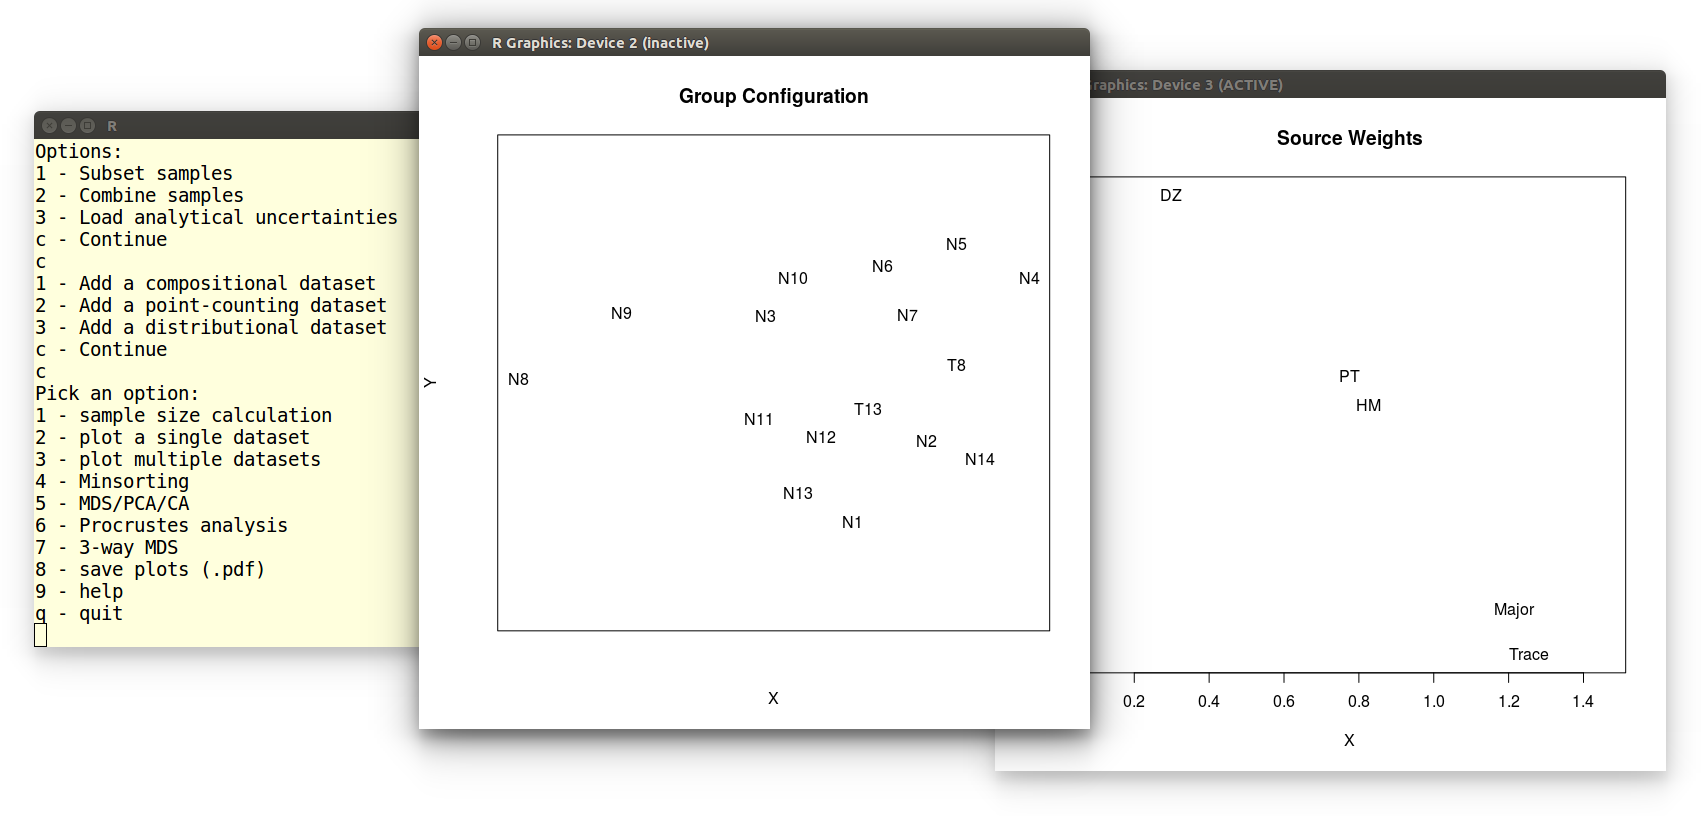
\includegraphics[width=\textwidth]{indscal.pdf}
  \caption{Output of the 3-way MDS analysis of Namib desert
    sand. Left: the group configurations shows the salient
    similarities and differences between samples as a `map' in which
    similar samples plot close together and dissimilar samples plot
    far apart. Right: the weights for each of the five data sources
    show that provenance proxies that are performed on the bulk
    sediment (e.g. the major and trace element compositions) attach a
    stronger weight to the X- than the y-axis. In contrast, proxies
    that are determined on specific density fractions (e.g. zircons,
    heavy minerals, or quartz -- feldspar -- lithics), attach stronger
    weight to the Y-axis. One geological interpretation of these
    dimensions is that samples that horizontally separated from each
    other on the group configuration (e.g., N4 and N8) have
    experienced hydraulic sorting, whereas samples that are vertically
    separated (e.g., N1 and N10) have a different provenance.}
  \label{fig:INDSCAL}
\end{figure}

\section{Summary, conclusions and outlook}
\label{sec:conclusions}

The statistical toolbox implemented by the \texttt{provenance} package
is neither comprehensive nor at the cutting edge of exploratory data
analysis. PCA, MDS, CA, and KDEs are tried and tested methods that
have been around for many decades.  Nothing new is presented here and
that is intentional. This paper makes the point that even the most
basic statistical parameters such as the arithmetic mean and standard
deviation cannot be blindly applied to geological data
\citep{chayes1949, chayes1960, weltje2002}. Great care must be taken
when applying established techniques to sedimentary provenance data
such as chemical compositions, point-counts or U-Pb age distributions.
Given the difficulty of using even the simplest of methods correctly,
geologists may want to think twice before exploring more complicated
methods, or inventing entirely new ones.\\

The set of tutorials presented in this paper did not cover all aspects
of statistical provenance analysis. Doing so would fill a book rather
than a paper. Some additional topics for such a book could include (1)
supervised and unsupervised learning algorithms such as cluster
analysis and discriminant analysis, which can group samples into
formal groups \citep{bhatia1983, bhatia1986, armstrong2005,
  tolosana2018}; (2) the physical and chemical processes that affect
the composition of sediment from `source to sink' \citep{allen2008,
  weltje2004, weltje2012, garzanti2018a}; and (3) quality checks and
corrections that must be made to ensure that the data reveal
meaningful provenance trends rather than sampling effects
\citep{garzanti2007, garzanti2009, resentini2013, malusa2013,
  malusa2019b}.\\

The paper introduced three distinct classes of provenance
data. Compositional, point-counting and distributional data each
require different statistical treatment. Multi-sample collections of
these data can be visualised by Multidimensional Scaling, using
different dissimilarity measures (Table~\ref{tab:3types}).
Distributional data can be compared using the Kolmogorov-Smirnov
statistic or related dissimilarity measures, and plugged straight into
an MDS algorithm for further inspection.  Compositional data such as
chemical concentrations can be visualised by conventional `normal'
statistics after logratio transformation.  The Euclidean distance in
logratio space is called the Aitchison distance in compositional data
space. Classical MDS using this distance is equivalent to Principal
Component Analysis.  Finally, point-counting data combine aspects of
compositional data analysis with multinomial sampling statistics. The
Chi-square distance is the natural way to quantify the dissimilarity
between multiple point-counting samples. MDS analysis using the
Chi-square distance is equivalent to Correspondence Analysis, which is
akin to PCA for categorical data.\\

However, there are some provenance proxies that do not easily fit into
these three categories. \emph{Varietal studies} using the chemical
composition of single grains of heavy minerals combine aspects of
compositional and distributional data \citep{morton1991,
  tolosana2018}. Similarly, paired U-Pb ages and Hf-isotope
compositions in zircon \citep{gerdes2006} do not easily fit inside the
distributional data class described above.  Using the tools provided
by the \texttt{provenance} package, such data can be processed by
procustes analysis or 3-way MDS (Section~\ref{sec:bigdata}). Thus,
U-Pb and $\epsilon$(Hf)-distributions, say, could be entered into the
\texttt{indscal} function as separate entities. However by doing so
the single-grain link between the two datasets would be
lost. Alternative approaches may be pursued to address this issue, and
new dissimilarity measures could be developed for this hybrid data
type.  Matrix decomposition may be a way forward in this direction
\citep{paatero1994, bloemsma2012, martinez2017}.

\begin{table}[!ht]
  \centering
  \captionsetup{width=.72\linewidth}
  \caption{A summary of the three types of provenance data introduced
    in this paper along with a suitable dissimilarity measure and its
    corresponding ordination technique.}
  \begin{tabular}{lll}
    data type & dissimilarity measure & ordination technique \\ \hline
    compositional & Aitchison & Principal Component Analysis \\
    point-counting & Chi-square & Correspondence Analysis  \\
    distributional & Kolmogorov-Smirnov & Multidimensional Scaling
  \end{tabular}
  \label{tab:3types}
\end{table}

\section*{Appendix: an introduction to \texttt{R}}
\label{sec:R}

\texttt{R} is an increasingly popular programming language for
scientific data processing. It is similar in scope and purpose to
\texttt{Matlab} but is available free of charge on any operating
system at \texttt{http://r-project.}\allowbreak\texttt{org}. A number
of different graphical user interfaces (GUIs) are available for
\texttt{R}, the most popular of which are \texttt{RGui},
\texttt{RStudio}, \texttt{RCommander} and \texttt{Tinn-R}.  For this
tutorial, however, the simple command line console suffices.

\begin{enumerate}
\item First, do some arithmetic:

%\begin{tcolorbox}
\begin{verbatim}
> 1 + 1
> sqrt(2)
> exp(log(10))
> 13%%5
\end{verbatim}
%\end{tcolorbox}

\noindent where the `\verb|>|' symbol marks the command prompt.

\item You can use the arrow to assign a value to a variable. Note that the
arrow can point both ways:

%\begin{tcolorbox}
\begin{verbatim}
> foo <- 2
> 4 -> bar
> foo <- foo*bar
\end{verbatim}
%\end{tcolorbox}

\item Create a sequence of values:

%\begin{tcolorbox}
\begin{verbatim}
> myvec <- c(2,4,6,8)
> myvec*2
\end{verbatim}
%\end{tcolorbox}

Query the third value of the vector:

%\begin{tcolorbox}
\begin{verbatim}
> myvec[3]
\end{verbatim}
%\end{tcolorbox}

Change the third value of the vector:

%\begin{tcolorbox}
\begin{verbatim}
> myvec[3] <- 100
\end{verbatim}
%\end{tcolorbox}

Change the second and the third value of the vector:

%\begin{tcolorbox}
\begin{verbatim}
> myvec[c(2,3)] <- c(100,101)
\end{verbatim}
%\end{tcolorbox}

Create a vector of 1, 2, 3, ..., 10:

%\begin{tcolorbox}
\begin{verbatim}
> seq(from=1,to=10,by=1)
\end{verbatim}
%\end{tcolorbox}

Equivalently:

%\begin{tcolorbox}
\begin{verbatim}
> seq(1,10,1)
> seq(1,10)
> seq(to=10,by=1,from=1)
> seq(to=10)
> 1:10
\end{verbatim}
%\end{tcolorbox}

Create a 10-element vector of twos:

%\begin{tcolorbox}
\begin{verbatim}
> rep(2,10)
\end{verbatim}
%\end{tcolorbox}

\item Create a 2 $\times$ 4 matrix of ones:

  %\begin{tcolorbox}
\begin{verbatim}
> mymat <- matrix(1,nrow=2,ncol=4)
\end{verbatim}
%\end{tcolorbox}

Change the third value in the first column of \texttt{mymat} to 3:

%\begin{tcolorbox}
\begin{verbatim}
> mymat[1,3] <- 3
\end{verbatim}
%\end{tcolorbox}

Change the entire second column of \texttt{mymat} to 2:

%\begin{tcolorbox}
\begin{verbatim}
> mymat[,2] <- 2
\end{verbatim}
%\end{tcolorbox}

The transpose of \texttt{mymat}:

%\begin{tcolorbox}
\begin{verbatim}
> t(mymat)
\end{verbatim}
%\end{tcolorbox}

Element-wise multiplication (\verb|*|) vs. matrix multiplication
(\verb|%*%|):

%\begin{tcolorbox}
\begin{verbatim}
> mymat * mymat
> mymat %*% t(mymat)
\end{verbatim}
%\end{tcolorbox}  

\item Lists are used to store more complex data objects:

%\begin{tcolorbox}
\begin{verbatim}
> mylist <- list(v=myvec, m=mymat, nine=9)
> mylist$v
\end{verbatim}
%\end{tcolorbox}

\item Plot the first against the second row of \texttt{mymat}:

%\begin{tcolorbox}
\begin{verbatim}
> plot(mymat[1,],mymat[2,],type='p')
\end{verbatim}
%\end{tcolorbox}

Draw lines between the points shown on the existing plot:

%\begin{tcolorbox}
\begin{verbatim}
> lines(mymat[1,],mymat[2,])
\end{verbatim}
%\end{tcolorbox}

Create a new plot with red lines but no points:

%\begin{tcolorbox}
\begin{verbatim}
> plot(mymat[1,],mymat[2,],type='l',col='red')
\end{verbatim}
%\end{tcolorbox}

Use a 1:1 aspect ratio for the X- and Y-axis:

%\begin{tcolorbox}
\begin{verbatim}
> plot(mymat[1,],mymat[2,],type='l',col='red',asp=1)
\end{verbatim}
%\end{tcolorbox}

\item Save the currently active plot as a vector-editable
  \texttt{.pdf} file:

%\begin{tcolorbox}
\begin{verbatim}
> dev.copy2pdf(file="trigonometry.pdf")
\end{verbatim}
%\end{tcolorbox}

\item To learn more about a function, type `\texttt{help}' or
  `\texttt{?}':

%\begin{tcolorbox}
\begin{verbatim}
> help(c)
> ?plot
\end{verbatim}
%\end{tcolorbox}

\item It is also possible to define one's own functions:

%\begin{tcolorbox}
\begin{verbatim}
> cube <- function(n){
>     return(n^3)
> }
\end{verbatim}
%\end{tcolorbox}

Using the newly created function:

%\begin{tcolorbox}
\begin{verbatim}
> cube(2)
> result <- cube(3)
\end{verbatim}
%\end{tcolorbox}

\item Create some random (uniform) numbers:

%\begin{tcolorbox}
\begin{verbatim}
> rand.num <- runif(100)
> hist(rand.num)
\end{verbatim}
%\end{tcolorbox}

\item List all the variables in the current workspace:

%\begin{tcolorbox}
\begin{verbatim}
> ls()
\end{verbatim}
%\end{tcolorbox}

Remove all the variables in the current workspace:

%\begin{tcolorbox}
\begin{verbatim}
> rm(list=ls())
\end{verbatim}
%\end{tcolorbox}

To get and set the working directory:
  
%\begin{tcolorbox}
\begin{verbatim}
> getwd()
> setwd("/path/to/a/valid/directory")
\end{verbatim}
%\end{tcolorbox}

\item Collect the following commands in a file called
  `\texttt{myscript.R}'.  Note that this text does not contain any
  `\verb|>|'-symbols because it is not entered at the command prompt
  but in a separate text editor:

%\begin{tcolorbox}[colback=blue!5!white]
\begin{verbatim}
# the 'print' function is needed to show intermediate
# results when running commands from an .R file
print(pi)
\end{verbatim}
%\end{tcolorbox}

This code can be run by going back to the command prompt (hence the
`\verb|>|' in the next box) and typing:

%\begin{tcolorbox}
\begin{verbatim}
> source("myscript.R")
\end{verbatim}
%\end{tcolorbox}

This should result in the number $\pi$ being printed to the console.
Note that everything that follows the `\verb|#|'-symbol was ignored by
\texttt{R}.

\item Conditional statements. Add the following function to
  \texttt{myscript.R}:

%\begin{tcolorbox}[colback=blue!5!white]
\begin{verbatim}
toss <- function(){
    if (runif(1)>0.5){
        print("head")
    } else {
        print("tail")
    }
}
\end{verbatim}
%\end{tcolorbox}

Save and run at the command prompt:

%\begin{tcolorbox}
\begin{verbatim}
> source('myscript.R')
> toss()
\end{verbatim}
%\end{tcolorbox}

\item Loops. Add the following function to \texttt{myscript.R}:

%\begin{tcolorbox}[colback=blue!5!white]
\begin{verbatim}
fibonnaci <- function(n){
    if (n < 3) { stop('n must be at least 3') }
    # seed the output vector with 0 and 1:
    s <- c(0,1)
    # loop through all numbers from 3 to n:
    for (i in 3:n){
        s[i] <- s[i-1] + s[i-2]
    }
    return(s)
}
\end{verbatim}
%\end{tcolorbox}

Save and run at the command prompt to calculate the first 20 numbers
in the Fibonnaci series:

%\begin{tcolorbox}
\begin{verbatim}
> source('myscript.R')
> fibonnaci(20)
\end{verbatim}
%\end{tcolorbox}

\item Arguably the greatest power of \texttt{R} is the availability of
  10,000 \textit{packages} that provide additional functionality. For
  example the \texttt{compositions} package implements a number of
  statistical tools for compositional data analysis
  \citep{vandenboogaart2008, vandenboogaart2013}.  To install this
  package:

%\begin{tcolorbox}
\begin{verbatim}
> install.packages('compositions')
\end{verbatim}
%\end{tcolorbox}

Use the newly installed package to plot the built-in \texttt{SkyeAFM}
dataset, which contains the Al\textsubscript{2}O\textsubscript{3} --
FeO -- MgO compositions of 23 aphyric lavas from the isle of Skye.

%\begin{tcolorbox}[colback=blue!5!white]
\begin{verbatim}
library(compositions) # load the package into memory
dat <- data(SkyeAFM)  # load the Skye lava dataset
AFMcomp <- acomp(dat) # enforce the constant sum constraint
plot(AFMcomp)         # plot as a ternary diagram
\end{verbatim}
%\end{tcolorbox}

Note that the \texttt{plot()} function has been \textit{overloaded}
for compositional data.

\end{enumerate}

\section*{Acknowledgments}

This paper evolved from a set of lecture notes for an iCRAG workshop
in sedimentary provenance analysis at NUI Galway.  The author would
like to thank Sergio And\`{o} for inviting him to contribute to this
Special Issue. The manuscript greatly benefited from three critical
but constructive reviews.

%\bibliographystyle{/home/pvermees/Dropbox/abbrvplainnat}
%\bibliography{/home/pvermees/Dropbox/biblio}

\begin{thebibliography}{68}
\providecommand{\natexlab}[1]{#1}
\providecommand{\url}[1]{\texttt{#1}}
\expandafter\ifx\csname urlstyle\endcsname\relax
  \providecommand{\doi}[1]{doi: #1}\else
  \providecommand{\doi}{doi: \begingroup \urlstyle{rm}\Url}\fi

\bibitem[Aitchison(1983)]{aitchison1983}
Aitchison, J.
\newblock Principal component analysis of compositional data.
\newblock \emph{Biometrika}, 70\penalty0 (1):\penalty0 57--65, 1983.
\newblock \doi{10.1093/biomet/70.1.57}.

\bibitem[Aitchison(1986)]{aitchison1986}
Aitchison, J.
\newblock \emph{The statistical analysis of compositional data}.
\newblock London, Chapman and Hall, 1986.

\bibitem[Aitchison and Brown(1957)]{aitchison1957}
Aitchison, J. and Brown, J.~A.
\newblock \emph{The lognormal distribution}.
\newblock Cambridge Univ. Press, 1957.
\newblock ISBN 0521040116.

\bibitem[Allen(2008)]{allen2008}
Allen, P.~A.
\newblock From landscapes into geological history.
\newblock \emph{Nature}, 451\penalty0 (7176):\penalty0 274, 2008.

\bibitem[Armstrong-Altrin and Verma(2005)]{armstrong2005}
Armstrong-Altrin, J. and Verma, S.~P.
\newblock {Critical evaluation of six tectonic setting discrimination diagrams
  using geochemical data of Neogene sediments from known tectonic settings}.
\newblock \emph{Sedimentary Geology}, 177\penalty0 (1-2):\penalty0 115--129,
  2005.

\bibitem[Bhatia(1983)]{bhatia1983}
Bhatia, M.~R.
\newblock Plate tectonics and geochemical composition of sandstones.
\newblock \emph{The Journal of Geology}, 91\penalty0 (6):\penalty0 611--627,
  1983.

\bibitem[Bhatia and Crook(1986)]{bhatia1986}
Bhatia, M.~R. and Crook, K.~A.
\newblock Trace element characteristics of graywackes and tectonic setting
  discrimination of sedimentary basins.
\newblock \emph{Contributions to mineralogy and petrology}, 92\penalty0
  (2):\penalty0 181--193, 1986.

\bibitem[Bloemsma and Weltje(2015)]{bloemsma2015}
Bloemsma, M.~R. and Weltje, G.~J.
\newblock {Reduced-rank approximations to spectroscopic and compositional data:
  A universal framework based on log-ratios and counting statistics}.
\newblock \emph{Chemometrics and Intelligent Laboratory Systems}, 142:\penalty0
  206--218, 2015.

\bibitem[Bloemsma et~al.(2012)Bloemsma, Zabel, Stuut, Tjallingii, Collins, and
  Weltje]{bloemsma2012}
Bloemsma, M., Zabel, M., Stuut, J., Tjallingii, R., Collins, J., and Weltje,
  G.~J.
\newblock Modelling the joint variability of grain size and chemical
  composition in sediments.
\newblock \emph{Sedimentary Geology}, 280:\penalty0 135--148, 2012.

\bibitem[{Botev} et~al.(2010){Botev}, {Grotowski}, and {Kroese}]{botev2010}
{Botev}, Z.~I., {Grotowski}, J.~F., and {Kroese}, D.~P.
\newblock {Kernel density estimation via diffusion}.
\newblock \emph{Annals of Statistics}, 38:\penalty0 2916--2957, 2010.

\bibitem[Carroll and Chang(1970)]{carroll1970}
Carroll, J.~D. and Chang, J.-J.
\newblock {Analysis of individual differences in multidimensional scaling via
  an N-way generalization of `Eckart-Young' decomposition}.
\newblock \emph{Psychometrika}, 35\penalty0 (3):\penalty0 283--319, 1970.

\bibitem[Chayes(1949)]{chayes1949}
Chayes, F.
\newblock On ratio correlation in petrography.
\newblock \emph{The Journal of Geology}, 57\penalty0 (3):\penalty0 239--254,
  1949.

\bibitem[Chayes(1960)]{chayes1960}
Chayes, F.
\newblock On correlation between variables of constant sum.
\newblock \emph{Journal of Geophysical research}, 65\penalty0 (12):\penalty0
  4185--4193, 1960.

\bibitem[Cox and Cox(2000)]{cox2000}
Cox, T.~F. and Cox, M.~A.
\newblock \emph{Multidimensional scaling}.
\newblock CRC Press, 2000.

\bibitem[de~Leeuw and Mair(2009)]{deleeuw2009}
de~Leeuw, J. and Mair, P.
\newblock {Multidimensional scaling using majorization: The R package smacof}.
\newblock \emph{Journal of Statistical Software}, 31\penalty0 (3):\penalty0
  1--30, 2009.
\newblock URL \url{http://www.jstatsoft.org/v31/i03/}.

\bibitem[DeGraaff-Surpless et~al.(2003)DeGraaff-Surpless, Mahoney, Wooden, and
  McWilliams]{degraaff2003}
DeGraaff-Surpless, K., Mahoney, J., Wooden, J., and McWilliams, M.
\newblock Lithofacies control in detrital zircon provenance studies: {I}nsights
  from the {C}retaceous {M}ethow basin, southern {C}anadian {C}ordillera.
\newblock \emph{Geological Society of America Bulletin}, 115:\penalty0
  899--915, 2003.
\newblock \doi{10.1130/B25267.1}.

\bibitem[DuToit et~al.(1986)DuToit, Steyn, and Stumpf]{dutoit1986}
DuToit, S.~H., Steyn, A. G.~W., and Stumpf, R.~H.
\newblock \emph{Graphical exploratory data analysis}.
\newblock Springer Science \& Business Media, 1986.

\bibitem[Fedo et~al.(2003)Fedo, Sircombe, and Rainbird]{fedo2003}
Fedo, C., Sircombe, K., and Rainbird, R.
\newblock Detrital zircon analysis of the sedimentary record.
\newblock \emph{Reviews in mineralogy and geochemistry}, 53:\penalty0 277--303,
  2003.

\bibitem[Feller(1948)]{feller1948}
Feller, W.
\newblock On the {K}olmogorov-{S}mirnov limit theorems for empirical
  distributions.
\newblock \emph{The Annals of Mathematical Statistics}, 19:\penalty0 177--189,
  1948.

\bibitem[Galbraith(1990)]{galbraith1990a}
Galbraith, R.~F.
\newblock The radial plot: graphical assessment of spread in ages.
\newblock \emph{Nuclear Tracks and Radiation Measurements}, 17:\penalty0
  207--214, 1990.

\bibitem[Galbraith(1988)]{galbraith1988}
Galbraith, R.
\newblock Graphical display of estimates having differing standard errors.
\newblock \emph{Technometrics}, 30\penalty0 (3):\penalty0 271--281, 1988.

\bibitem[Garzanti and And{\`{o}}(2007)]{garzanti2007}
Garzanti, E. and And{\`{o}}, S.
\newblock Heavy-mineral concentration in modern sands: implications for
  provenance interpretation.
\newblock In Mange, M. and Wright, D., editors, \emph{Heavy Minerals in Use,
  {D}evelopments in {S}edimentology {S}eries 58}, pages 517--545. Elsevier,
  Amsterdam, 2007.

\bibitem[{Garzanti} et~al.(2009){Garzanti}, {And{\`o}}, and
  {Vezzoli}]{garzanti2009}
{Garzanti}, E., {And{\`o}}, S., and {Vezzoli}, G.
\newblock {Grain-size dependence of sediment composition and environmental bias
  in provenance studies}.
\newblock \emph{Earth and Planetary Science Letters}, 277:\penalty0 422--432,
  2009.
\newblock \doi{10.1016/j.epsl.2008.11.007}.

\bibitem[Garzanti(2019)]{garzanti2019}
Garzanti, E.
\newblock Petrographic classification of sand and sandstone.
\newblock \emph{Earth-Science Reviews}, 2019.
\newblock \doi{10.1016/j.earscirev.2018.12.014}.

\bibitem[Garzanti et~al.(2018)Garzanti, Dinis, Vermeesch, And{\`o}, Hahn, Huvi,
  Limonta, Padoan, Resentini, Rittner, and Vezzoli]{garzanti2018a}
Garzanti, E., Dinis, P., Vermeesch, P., And{\`o}, S., Hahn, A., Huvi, J.,
  Limonta, M., Padoan, M., Resentini, A., Rittner, M., and Vezzoli, G.
\newblock {Sedimentary processes controlling ultralong cells of littoral
  transport: Placer formation and termination of the Orange sand highway in
  southern Angola}.
\newblock \emph{Sedimentology}, 65\penalty0 (2):\penalty0 431--460, 2018.

\bibitem[Gehrels(2011)]{gehrels2011}
Gehrels, G.
\newblock {Detrital zircon U-Pb geochronology: Current methods and new
  opportunities}.
\newblock In Busby, C. and Azor, A., editors, \emph{Tectonics of sedimentary
  basins: Recent advances}, chapter~2, pages 45--62. Wiley Online Library,
  2011.

\bibitem[Gerdes and Zeh(2006)]{gerdes2006}
Gerdes, A. and Zeh, A.
\newblock {Combined U--Pb and Hf isotope LA-(MC-) ICP-MS analyses of detrital
  zircons: comparison with SHRIMP and new constraints for the provenance and
  age of an Armorican metasediment in Central Germany}.
\newblock \emph{Earth and Planetary Science Letters}, 249\penalty0
  (1-2):\penalty0 47--61, 2006.

\bibitem[Gower(1975)]{gower1975}
Gower, J.~C.
\newblock Generalized procrustes analysis.
\newblock \emph{Psychometrika}, 40\penalty0 (1):\penalty0 33--51, 1975.

\bibitem[Greenacre(1984)]{greenacre1984}
Greenacre, M.~J.
\newblock \emph{Theory and applications of correspondence analysis}.
\newblock Academic Press, 1984.

\bibitem[Kenkel(2006)]{kenkel2006}
Kenkel, N.
\newblock On selecting an appropriate multivariate analysis.
\newblock \emph{Canadian Journal of Plant Science}, 86\penalty0 (3):\penalty0
  663--676, 2006.

\bibitem[Kenkel and Orl{\'o}ci(1986)]{kenkel1986}
Kenkel, N.~C. and Orl{\'o}ci, L.
\newblock Applying metric and nonmetric multidimensional scaling to ecological
  studies: some new results.
\newblock \emph{Ecology}, pages 919--928, 1986.

\bibitem[Kruskal and Wish(1978)]{kruskal1978}
Kruskal, J.~B. and Wish, M.
\newblock \emph{Multidimensional scaling}, volume 07-011 of \emph{Sage
  University Paper series on Quantitative Application in the Social Sciences}.
\newblock Sage Publications, Beverly Hills and London, 1978.

\bibitem[Le~Maitre et~al.(2002)Le~Maitre, Streckeisen, Zanettin, Le~Bas, Bonin,
  and Bateman]{lemaitre2002}
Le~Maitre, R.~W., Streckeisen, A., Zanettin, B., Le~Bas, M., Bonin, B., and
  Bateman, P.
\newblock \emph{{Igneous rocks: a classification and glossary of terms:
  recommendations of the International Union of Geological Sciences
  Subcommission on the Systematics of Igneous Rocks}}.
\newblock Cambridge University Press, 2002.
\newblock ISBN 9780511535581.

\bibitem[Malus{\`a} and Garzanti(2019)]{malusa2019b}
Malus{\`a}, M.~G. and Garzanti, E.
\newblock The sedimentology of detrital thermochronology.
\newblock In \emph{Fission-Track Thermochronology and its Application to
  Geology}, pages 123--143. Springer, 2019.

\bibitem[Malus{\`a} et~al.(2013)Malus{\`a}, Carter, Limoncelli, Villa, and
  Garzanti]{malusa2013}
Malus{\`a}, M.~G., Carter, A., Limoncelli, M., Villa, I.~M., and Garzanti, E.
\newblock Bias in detrital zircon geochronology and thermochronometry.
\newblock \emph{Chemical Geology}, 359:\penalty0 90--107, 2013.

\bibitem[Malus{\`a} et~al.(2016)Malus{\`a}, Resentini, and
  Garzanti]{malusa2016}
Malus{\`a}, M.~G., Resentini, A., and Garzanti, E.
\newblock Hydraulic sorting and mineral fertility bias in detrital
  geochronology.
\newblock \emph{Gondwana Research}, 31:\penalty0 1--19, 2016.

\bibitem[Mart{\'\i}n-Fern{\'a}ndez et~al.(2003)Mart{\'\i}n-Fern{\'a}ndez,
  Barcel{\'o}-Vidal, and Pawlowsky-Glahn]{martin2003}
Mart{\'\i}n-Fern{\'a}ndez, J.~A., Barcel{\'o}-Vidal, C., and Pawlowsky-Glahn,
  V.
\newblock Dealing with zeros and missing values in compositional data sets
  using nonparametric imputation.
\newblock \emph{Mathematical Geology}, 35\penalty0 (3):\penalty0 253--278,
  2003.

\bibitem[Martinez et~al.(2017)Martinez, Martinez, and Solka]{martinez2017}
Martinez, W.~L., Martinez, A.~R., and Solka, J.
\newblock \emph{{Exploratory data analysis with MATLAB}}.
\newblock Chapman and Hall/CRC, 2017.
\newblock ISBN 9781498776066.

\bibitem[Mazumder(2017)]{mazumder2017}
Mazumder, R.
\newblock Sediment provenance.
\newblock In Mazumder, R., editor, \emph{Sediment Provenance: Influence on
  Compositional Change From Source to Sink}, pages 1--4. Elsevier, 2017.

\bibitem[Morton(1991)]{morton1991}
Morton, A.~C.
\newblock Geochemical studies of detrital heavy minerals and their application
  to provenance research.
\newblock In Morton, A., Todd, S., and Haughton, P. D.~W., editors,
  \emph{{Developments in Sedimentary Provenance Studies}}, volume~57, pages
  31--45. Geological Society of London, 1991.

\bibitem[Morton and Hallsworth(1999)]{morton1999}
Morton, A.~C. and Hallsworth, C.~R.
\newblock Processes controlling the composition of heavy mineral assemblages in
  sandstones.
\newblock \emph{Sedimentary Geology}, 124\penalty0 (1-4):\penalty0 3--29, 1999.

\bibitem[Nesbitt and Young(1989)]{nesbitt1989}
Nesbitt, H. and Young, G.~M.
\newblock Formation and diagenesis of weathering profiles.
\newblock \emph{The Journal of Geology}, 97\penalty0 (2):\penalty0 129--147,
  1989.

\bibitem[Paatero and Tapper(1994)]{paatero1994}
Paatero, P. and Tapper, U.
\newblock {Positive matrix factorization: A non-negative factor model with
  optimal utilization of error estimates of data values}.
\newblock \emph{Environmetrics}, 5\penalty0 (2):\penalty0 111--126, 1994.

\bibitem[Pawlowsky-Glahn et~al.(2015)Pawlowsky-Glahn, Egozcue, and
  Tolosana-Delgado]{pawlowsky2015}
Pawlowsky-Glahn, V., Egozcue, J.~J., and Tolosana-Delgado, R.
\newblock \emph{Modeling and analysis of compositional data}.
\newblock John Wiley \& Sons, 2015.

\bibitem[Pearson(1901)]{pearson1901}
Pearson, K.
\newblock On lines and planes of closest fit to systems of points in space.
\newblock \emph{The London, Edinburgh, and Dublin Philosophical Magazine and
  Journal of Science}, 2\penalty0 (11):\penalty0 559--572, 1901.

\bibitem[Resentini et~al.(2013)Resentini, Malus{\`a}, and
  Garzanti]{resentini2013}
Resentini, A., Malus{\`a}, M.~G., and Garzanti, E.
\newblock {MinSORTING: An Excel{\textregistered} worksheet for modelling
  mineral grain-size distribution in sediments, with application to detrital
  geochronology and provenance studies}.
\newblock \emph{Computers \& Geosciences}, 59:\penalty0 90--97, 2013.

\bibitem[Ripley(2002)]{ripley2002}
Ripley, B.
\newblock {Modern applied statistics with S}.
\newblock \emph{Statistics and Computing, fourth ed. Springer, New York}, 2002.

\bibitem[Rittner et~al.(2016)Rittner, Vermeesch, Carter, Bird, Stevens,
  Garzanti, And\`{o}, Vezzoli, Dutt, Xu, and Lu]{rittner2016}
Rittner, M., Vermeesch, P., Carter, A., Bird, A., Stevens, T., Garzanti, E.,
  And\`{o}, S., Vezzoli, G., Dutt, R., Xu, Z., and Lu, H.
\newblock {The provenance of Taklamakan desert sand}.
\newblock \emph{Earth and Planetary Science Letters}, 437:\penalty0 127 -- 137,
  2016.
\newblock ISSN 0012-821X.

\bibitem[Shepard(1962)]{shepard1962}
Shepard, R.~N.
\newblock The analysis of proximities: multidimensional scaling with an unknown
  distance function. i.
\newblock \emph{Psychometrika}, 27\penalty0 (2):\penalty0 125--140, 1962.

\bibitem[Silverman(1986)]{silverman1986}
Silverman, B.
\newblock \emph{Density Estimation for Statistics and Data Analysis}.
\newblock Chapman and Hall, London, 1986.

\bibitem[Stephan et~al.(2018)Stephan, Kroner, and Romer]{stephan2018}
Stephan, T., Kroner, U., and Romer, R.~L.
\newblock The pre-orogenic detrital zircon record of the peri-gondwanan crust.
\newblock \emph{Geological Magazine}, pages 1--27, 2018.

\bibitem[Tolosana-Delgado et~al.(2018)Tolosana-Delgado, von Eynatten, Krippner,
  and Meinhold]{tolosana2018}
Tolosana-Delgado, R., von Eynatten, H., Krippner, A., and Meinhold, G.
\newblock A multivariate discrimination scheme of detrital garnet chemistry for
  use in sedimentary provenance analysis.
\newblock \emph{Sedimentary Geology}, 375:\penalty0 14--26, 2018.

\bibitem[Torgerson(1952)]{torgerson1952}
Torgerson, W.~S.
\newblock {Multidimensional scaling: I. Theory and method}.
\newblock \emph{Psychometrika}, 17\penalty0 (4):\penalty0 401--419, 1952.

\bibitem[Tukey(1977)]{tukey1977}
Tukey, J.~W.
\newblock \emph{Exploratory data analysis}, volume~2.
\newblock Addison-Wesley, 1977.
\newblock ISBN 978-0-201-07616-5.

\bibitem[Van~den Boogaart and Tolosana-Delgado(2008)]{vandenboogaart2008}
Van~den Boogaart, K.~G. and Tolosana-Delgado, R.
\newblock ``{C}ompositions'': a unified {R} package to analyze compositional
  data.
\newblock \emph{Computers \& Geosciences}, 34\penalty0 (4):\penalty0 320--338,
  2008.

\bibitem[Van~den Boogaart and Tolosana-Delgado(2013)]{vandenboogaart2013}
Van~den Boogaart, K.~G. and Tolosana-Delgado, R.
\newblock \emph{{Analyzing compositional data with R}}, volume 122 of
  \emph{UseR!}
\newblock Springer, 2013.

\bibitem[Van~der Plas and Tobi(1965)]{vanderplas1965}
Van~der Plas, L. and Tobi, A.
\newblock A chart for judging the reliability of point counting results.
\newblock \emph{American Journal of Science}, 263\penalty0 (1):\penalty0
  87--90, 1965.

\bibitem[Vermeesch(2007)]{vermeesch2007a}
Vermeesch, P.
\newblock {Quantitative geomorphology of the White Mountains (California) using
  detrital apatite fission track thermochronology}.
\newblock \emph{Journal of Geophysical Research (Earth Surface)}, 112\penalty0
  (F11):\penalty0 3004, 2007.
\newblock \doi{10.1029/2006JF000671}.

\bibitem[Vermeesch(2012)]{vermeesch2012b}
Vermeesch, P.
\newblock On the visualisation of detrital age distributions.
\newblock \emph{Chemical Geology}, 312-313:\penalty0 190--194, 2012.
\newblock \doi{10.1016/j.chemgeo.2012.04.021}.

\bibitem[Vermeesch(2013)]{vermeesch2013}
Vermeesch, P.
\newblock Multi-sample comparison of detrital age distributions.
\newblock \emph{Chemical Geology}, 341:\penalty0 140--146, 2013.

\bibitem[Vermeesch(2018{\natexlab{a}})]{vermeesch2018b}
Vermeesch, P.
\newblock {Dissimilarity measures in detrital geochronology}.
\newblock \emph{Earth-Science Reviews}, 178:\penalty0 310--321,
  2018{\natexlab{a}}.
\newblock \doi{10.1016/j.earscirev.2017.11.027}.

\bibitem[Vermeesch(2018{\natexlab{b}})]{vermeesch2018d}
Vermeesch, P.
\newblock Statistical models for point-counting data.
\newblock \emph{Earth and Planetary Science Letters}, 501:\penalty0 1--7,
  2018{\natexlab{b}}.

\bibitem[Vermeesch and Garzanti(2015)]{vermeesch2015}
Vermeesch, P. and Garzanti, E.
\newblock {Making geological sense of `Big Data' in sedimentary provenance
  analysis}.
\newblock \emph{Chemical Geology}, 409:\penalty0 20--27, 2015.

\bibitem[Vermeesch et~al.(2016)Vermeesch, Resentini, and
  Garzanti]{vermeesch2016a}
Vermeesch, P., Resentini, A., and Garzanti, E.
\newblock {An R package for statistical provenance analysis}.
\newblock \emph{Sedimentary Geology}, 2016.

\bibitem[Weltje(2012)]{weltje2012}
Weltje, G.~J.
\newblock {Quantitative models of sediment generation and provenance: state of
  the art and future developments}.
\newblock \emph{Sedimentary Geology}, 280:\penalty0 4--20, 2012.

\bibitem[Weltje and von Eynatten(2004)]{weltje2004}
Weltje, G.~J. and von Eynatten, H.
\newblock Quantitative provenance analysis of sediments: review and outlook.
\newblock \emph{Sedimentary Geology}, 171\penalty0 (1-4):\penalty0 1--11, 2004.

\bibitem[Weltje(2002)]{weltje2002}
Weltje, G.
\newblock Quantitative analysis of detrital modes: statistically rigorous
  confidence regions in ternary diagrams and their use in sedimentary
  petrology.
\newblock \emph{Earth-Science Reviews}, 57\penalty0 (3-4):\penalty0 211 -- 253,
  2002.
\newblock ISSN 0012-8252.
\newblock \doi{DOI: 10.1016/S0012-8252(01)00076-9}.

\bibitem[Young and Householder(1938)]{young1938}
Young, G. and Householder, A.~S.
\newblock Discussion of a set of points in terms of their mutual distances.
\newblock \emph{Psychometrika}, 3\penalty0 (1):\penalty0 19--22, 1938.

\end{thebibliography}


\end{document}
